%%
%% Copyright 2007, 2008, 2009 Elsevier Ltd
%%
%% This file is part of the 'Elsarticle Bundle'.
%% ---------------------------------------------
%%
%% It may be distributed under the conditions of the LaTeX Project Public
%% License, either version 1.2 of this license or (at your option) any
%% later version.  The latest version of this license is in
%%    http://www.latex-project.org/lppl.txt
%% and version 1.2 or later is part of all distributions of LaTeX
%% version 1999/12/01 or later.
%%
%% The list of all files belonging to the 'Elsarticle Bundle' is
%% given in the file `manifest.txt'.
%%

%% Template article for Elsevier's document class `elsarticle'
%% with numbered style bibliographic references
%% SP 2008/03/01
%%
%%
%%
%% $Id: elsarticle-template-num.tex 4 2009-10-24 08:22:58Z rishi $
%%alignat
%%
%\documentclass[review,12pt]{elsarticle}
\documentclass[final,3p,times]{elsarticle}
\usepackage[fleqn]{amsmath}
\usepackage{graphicx}
\usepackage{float}
\usepackage{amsfonts}
\usepackage{enumitem}
\usepackage{amsmath}
\usepackage{mathtools}
\usepackage{amssymb}
\usepackage{amsthm}
\usepackage{multicol}
\usepackage{multirow}
\usepackage{url}
\usepackage{bm}
\usepackage{enumitem}
\usepackage{booktabs}
\usepackage{siunitx}
\usepackage{subcaption}
\usepackage{algorithm,algorithmic}
\usepackage{color}
\usepackage[colorlinks=true, linkcolor=blue, urlcolor=black,citecolor=blue]{hyperref}
% % you should run this command for nomenclature
% makeindex ArmanManuscriptMultiphase.nlo -s nomencl.ist -o ArmanManuscriptMultiphase.nls
\usepackage[toc,page]{appendix}

\usepackage{framed}
\usepackage{mdwlist}

\usepackage{tikz}
\usepackage{pgfplots}
\usetikzlibrary{shapes,arrows,shadows}

%\usetikzlibrary{external}
%\tikzexternalize
%\tikzsetexternalprefix{tikz/}
%\tikzset{external/up to date check=diff}

%  Notes command (uncomment the first for publication, uncomment the second
%  when working on the paper)

%\definecolor{darkgreen}{rgb}{0,0.4,0}


%\newcommand{\CHRONO}{{\sffamily{{Chrono}}}\xspace}
\newcommand{\CHRONO}{{\sffamily{{Chrono}}}}
\newcommand{\softpackage}[1]{{\sffamily{#1}}}
\newcommand*{\rom}[1]{\expandafter\@slowromancap\romannumeral #1@}
\def\mathbbm#1{\mathbb{#1}}% ***ALEX***
%\def\vect#1{{\bf #1}}
\def\amatr#1{{\bf #1}}

\newcommand\todo[1]{{\textcolor{red}{\bf{#1}}}}

\newcommand{\cA}{{\cal A}}
\newcommand{\cL}{{\cal L}}
\newcommand{\cone}{{\Upsilon}}
\newcommand{\cD}{{\cal D}}

\newcommand{\BigPT}{{{\bf D}^T}}
\newcommand{\BigP}{{{\bf D}}}
\newcommand{\ProjT}[1]{\,{{\bf D}}^T_{#1}}
\newcommand{\Proj}[1]{\,{{\bf D}}_{#1}}
\newcommand{\Pn}[1]{\,{{\bf D}}_{#1,{n}}}
\newcommand{\Ptu}[1]{\,{{\bf D}}_{#1,{u}}}
\newcommand{\Ptw}[1]{\,{{\bf D}}_{#1,{w}}}
\newcommand{\PnT}[1]{\,{{\bf D}}^T_{#1,{n}}}
\newcommand{\PtuT}[1]{\,{{\bf D}}^T_{#1,{u}}}
\newcommand{\PtwT}[1]{\,{{\bf D}}^T_{#1,{w}}}

\newcommand{\CP}[1]{{{\Pi}_{{\cone}_{#1}}}}

\newcommand{\nVec}[1]{{\bf n}_{#1}}
\newcommand{\uVec}[1]{{\bf u}_{#1}}
\newcommand{\wVec}[1]{{\bf w}_{#1}}

\newcommand{\hatGN}[1]{{\widehat{\gamma}_{#1,n}}}
\newcommand{\hatGU}[1]{{\widehat{\gamma}_{#1,u}}}
\newcommand{\hatGW}[1]{{\widehat{\gamma}_{#1,w}}}
\newcommand{\hatGB}[1]{{\widehat{\gamma}_{#1,b}}}

\newcommand{\BigG}{{\bf \gamma}}
\newcommand{\Gt}[1]{{{\bf \gamma}^{T}_{#1}}}
\newcommand{\GN}[1]{{{\gamma}_{#1,n}}}
\newcommand{\GU}[1]{{{\gamma}_{#1,u}}}
\newcommand{\GW}[1]{{{\gamma}_{#1,w}}}
\newcommand{\GB}[1]{{{\gamma}_{#1,b}}}
\newcommand{\GUsq}[1]{{{\gamma}}^2_{#1,u}}
\newcommand{\GWsq}[1]{{{\gamma}}^2_{#1,w}}
\newcommand{\itG}[2]{{{\gamma}^{(#2)}_{#1}}}

\newcommand{\norm}[1]{{ \left| { \left| #1 \right| }  \right| }}
\newcommand{\subVect}[2]{{#1}_{{#2}}}

\newcommand{\vect}[1]{\boldsymbol{#1}}
\newcommand{\matr}[1]{\boldsymbol{#1}}
\DeclareMathOperator*{\argmin}{arg\,min}


%\newcommand{\R}{\mathbb{R}}
\newcommand{\R}{\Re}
\newcommand{\row}{\Re^{1 \times 3}}
\newcommand{\col}{\Re^{3}}
\newcommand{\mat}{\Re^{3 \times 3}}

%\newcommand{\br}{{\bf r}}
%\newcommand{\bv}{{\bf v}}
\newcommand{\bp}{{\bf p}}
%\newcommand{\bx}{{\bf x}}
\newcommand{\by}{{\bf y}}
\newcommand{\bz}{{\bf z}}

\newcommand{\bJW}{{\bf J}_W}
\newcommand{\X}{{\boldsymbol \xi}_a}
\newcommand{\Z}{{\boldsymbol \zeta}_a}
%\newcommand{\C}{{\chi}_a}

\newcommand{\qr}{q_{\bf r}}
\newcommand{\qrr}{q_{\bf rr}}

\newcommand{\nablaT}{\nabla^T}
\newcommand{\nablaa}{\nabla_a}
\newcommand{\nablab}{\nabla_b}
\newcommand{\nablaaT}{\nabla_a^T}
\newcommand{\nablabT}{\nabla_b^T}

\newcommand{\p}{\partial}
\newcommand{\pr}{\partial_{\bf r}}
\newcommand{\pra}{\partial_{{\bf r}_a}}
\newcommand{\prb}{\partial_{{\bf r}_b}}
\newcommand{\pva}{\partial_{{\bf v}_a}}
\newcommand{\pvb}{\partial_{{\bf v}_b}}
\newcommand{\ppa}{\partial_{p_a}}
\newcommand{\ppb}{\partial_{p_b}}
%-------------------------------------------------------
\newcommand{\bM}{\mathbf{M}}
\newcommand{\bQ}{\mathbf{Q}}
\newcommand{\bS}{\mathbf{S}}
\newcommand{\bI}{\mathbf{I}}
\newcommand{\bJ}{\mathbf{J}}
\newcommand{\bG}{\mathbf{G}}
\newcommand{\bT}{\mathbf{T}}
\newcommand{\bV}{\mathbf{V}}
\newcommand{\bX}{\mathbf{X}}
\newcommand{\bepsilon}{\mathbf{\epsilon}}
\newcommand{\bsigma}{\mathbf{\sigma}}
\newcommand{\ba}{\mathbf{a}}
\newcommand{\br}{\mathbf{r}}
\newcommand{\bv}{\mathbf{v}}
\newcommand{\xv}{\hat{\bv}}
\newcommand{\bff}{\mathbf{f}}
\newcommand{\bs}{\mathbf{s}}
\newcommand{\bt}{\mathbf{t}}
\newcommand{\brho}{\boldsymbol\rho}
\newcommand{\bomega}{\boldsymbol\omega}
%\newcommand{\xva}{\left\langle {{\bv_a}} \right\rangle}
\newcommand{\be}{\mathbf{e}}
\newcommand{\bx}{\mathbf{x}}
\newcommand{\bq}{\mathbf{q}}
\newcommand{\bu}{\mathbf{u}}
\newcommand{\bef}{\mathbf{f}}
\newcommand{\bn}{\mathbf{n}}
\newcommand{\VO}{\mathbb{V}}
\newcommand{\AR}{\mathbb{A}}
%\newcommand{\dd}{\mathrm{d}}
\newcommand{\dd}{d}
%cek
\newcommand{\support}[1]{\mathbf{supp}(#1)}
%\input{../../../SBEL-LaTeX/Macros/macrosSBEL}
%\input{macrosSBEL}

%\usepackage{tikz}
%%\usetikzlibrary{external}
%%\tikzexternalize
%%\tikzsetexternalprefix{tikz/}
%\usepackage{pgfplots}
%\usepackage{pgfplotstable}

\newcommand{\bg}{\mathbf{g}}
%\newcommand{\xva}{\left\langle {{\bv_a}} \right\rangle}
\newcommand{\nFluid}{{N_F}}                      % number of SPH fluid particles 
\newcommand{\V}{\mathbb{V}}
\newcommand{\A}{\mathbb{A}}
\newcommand{\SBELfeedback}[2]{{\bf{\textcolor{red}{#1}}} {\textcolor{blue}{(#2)}}}
\newcommand{\RN}[1]{%
	\textup{\expandafter{\romannumeral#1}}%
}
\newcommand{\sign}{\text{sign}}
\newcommand{\cek}[1]{{\bf{\textcolor{red}{#1}}}}
\usepackage{dsfont}
\usepackage{marginnote}
\renewcommand*{\marginfont}{\color{red}\sffamily}
\newcommand\Rey{\mbox{\textit{Re}}}
%% Use the option review to obtain double line spacing
%% \documentclass[preprint,review,12pt]{elsarticle}

%% Use the options 1p,twocolumn; 3p; 3p,twocolumn; 5p; or 5p,twocolumn
%% for a journal layout:
% \documentclass[final,1p,times]{elsarticle}
%% \documentclass[final,1p,times,twocolumn]{elsarticle}
%% \documentclass[final,3p,times]{elsarticle}
%% \documentclass[final,3p,times,twocolumn]{elsarticle}
%% \documentclass[final,5p,times]{elsarticle}
%% \documentclass[final,5p,times,twocolumn]{elsarticle}

%% if you use PostScript figures in your article
%% use the graphics package for simple commands
%% \usepackage{graphics}
%% or use the graphicx package for more complicated commands
%% \usepackage{graphicx}
%% or use the epsfig package if you prefer to use the old commands
%% \usepackage{epsfig}

%% The amssymb package provides various useful mathematical symbols
%\usepackage{amssymb}
%\usepackage{amsmath}
%% The amsthm package provides extended theorem environments
%% \usepackage{amsthm}

%% The lineno packages adds line numbers. Start line numbering with
%% \begin{linenumbers}, end it with \end{linenumbers}. Or switch it on
%% for the whole article with \linenumbers after \end{frontmatter}.
%% \usepackage{lineno}

%% natbib.sty is loaded by default. However, natbib options can be
%% provided with \biboptions{...} command. Following options are
%% valid:

%%   round  -  round parentheses are used (default)
%%   square -  square brackets are used   [option]
%%   curly  -  curly braces are used      {option}
%%   angle  -  angle brackets are used    <option>
%%   semicolon  -  multiple citations separated by semi-colon
%%   colon  - same as semicolon, an earlier confusion
%%   comma  -  separated by comma
%%   numbers-  selects numerical citations
%%   super  -  numerical citations as superscripts
%%   sort   -  sorts multiple citations according to order in ref. list
%%   sort&compress   -  like sort, but also compresses numerical citations
%%   compress - compresses without sorting
%%
%% \biboptions{comma,round}

% \biboptions{}

%\biboptions{sort&compress}

\journal{Computer Physics Communications}

\begin{document}

\begin{frontmatter}

%% Title, authors and addresses

%% use the tnoteref command within \title for footnotes;
%% use the tnotetext command for the associated footnote;
%% use the fnref command within \author or \address for footnotes;
%% use the fntext command for the associated footnote;
%% use the corref command within \author for corresponding author footnotes;
%% use the cortext command for the associated footnote;
%% use the ead command for the email address,
%% and the form \ead[url] for the home page:
%%
%% \title{Title\tnoteref{label1}}
%% \tnotetext[label1]{}
%% \author{Name\corref{cor1}\fnref{label2}}
%% \ead{email address}
%% \ead[url]{home page}
%% \fntext[label2]{}
%% \cortext[cor1]{}
%% \address{Address\fnref{label3}}
%% \fntext[label3]{}

\title{Lagrangian vs. Eulerian: An Analysis of Two Solution Methods for Free-Surface Flows and Fluid Solid Interaction Problems}

%% use optional labels to link authors explicitly to addresses:
%% \author[label1,label2]{<author name>}
%% \address[label1]{<address>}
%% \address[label2]{<address>}

\address[UWMadison]{Department of Mechanical Engineering, University of Wisconsin-Madison, Madison, WI 53706, USA}
\address[LSU]{Department of Civil \& Environmental Engineering, 3240P Patrick F. Taylor Hall, Louisiana State University, Baton Rouge, LA 70803}
\author[UWMadison]{M.~Rakhsha}
\ead{rakhsha@wisc.edu}
\author[LSU]{C.E.~Kees}
\ead{cekees@lsu.edu }
\author[UWMadison,cor1]{D.~Negrut}
\ead{negrut@wisc.edu}
\cortext[cor1]{Corresponding author: Dan Negrut}

\begin{abstract}
As a step towards addressing a scarcity of references on this topic, we compare the Eulerian and Lagrangian Computational Fluid Dynamics (CFD) approaches for the solution of free-surface and Fluid-Solid Interaction (FSI) problems. The Eulerian approach uses the Finite Element Method (FEM) to spatially discretize the Navier-Stokes equations. The free surface is handled via the volume of fluid (VOF) and the level set (LS) equations; an Immersed Boundary Method (IBM) in conjunction with the Nitsche's technique are applied to resolve the fluid-solid coupling. For the Lagrangian approach, the smoothed particle hydrodynamics (SPH) method is the meshless discretization technique of choice; no additional equations are needed to handle free-surface or FSI coupling. We compare the two approaches for a flow around cylinder. The dam break test is used to gauge performance for free-surface flows. Lastly, the two approaches are compared on two FSI problems -- one with a floating rigid body dropped into the fluid and one with an elastic gate interacting with the flow. We conclude with a discussion of the robustness, ease of model setup, and versatility of the two approaches. The Eulerian and Lagrangian solvers used in this study are open-source and available in the public domain.
\end{abstract}

\begin{keyword}
%% keywords here, in the form: keyword \sep keyword

%% MSC codes here, in the form: \MSC code \sep code
%% or \MSC[2008] code \sep code (2000 is the default)
Computational Fluid Dynamics \sep fluid solid interaction  \sep free-surface \sep Eulerian method \sep Lagrangian method
\end{keyword}

\end{frontmatter}

%% main text
\section{Introduction}
\label{sec:Introduction}


Insofar as the space discretization step is concerned, the majority of CFD models can be classified as : $(i)$ Eulerian approaches, where the unknown state variables are attached to stationary observers; or $(ii)$ Lagrangian approaches, in which the unknown state variables are attached to moving observers. The two approaches are vastly different and this contribution's goal is to shed light onto how they compare when used in conjunction with 3D applications that involve interactions with the solid phase.

Eulerian methods have been successfully applied and are very popular in CFD. Indeed, Finite Difference (FD) represents a robust technique for solving partial differential equations on simple domains, while the Finite Volume (FV) has been predominantly applied in fluid flows with complex geometries. Conversely, the Lagrangian methods gained traction only about two decades ago although the idea of using Lagrangian discretization dates back to 1957 \cite{PIC}. Among Lagrangian methods, SPH  \cite{Lucy1977,Gingold1977} has been widely adopted as the low-order approximation of choice for a variety of problems \cite{Monaghan2005a}, while Moving Least Squares and Radial Basis Functions emerged as the leading high-order meshless methods \cite{trask2016compact,hu2019spatially,trask2018compatible,kansa1990scattered}. 

For the class of free-surface flows, Eulerian approaches rely on either interface-tracking or interface-capturing techniques. The former is considered more accurate yet it involves an update stage in the computational mesh as the shape of the spatial domain occupied by the fluid changes in time. The latter is more flexible in terms of meshing, since the solution relies on one fixed spatial grid that contains two fluid phases. Owing to the introduction of two distinct phases, interface-capturing methods require the solution of additional equations governing the advection of the interface and/or conservation of the phase fraction \cite{tezduyar2006interface,Hirt1981,SSO94,SP00}. The ability to handle two distinct phases is critical in many practical applications in which two or more fluids with different viscosities and densities play equally important roles in the problem, e.g. in the oil and gas industries. On the other hand, handling free-surface problems is more straightforward in Lagrangian approaches. Owing to their meshless nature, these methods eschew the costly re-meshing requirement of interface-tracking methods.  

For FSI problems, just as for free-surface flows, the Eulerian approaches are challenged by large mesh deformations, which call upon remeshing operations. A widely used approach is the Arbitrary Lagrangian-Eulerian (ALE) method \cite{ALE1974}, which handles well sufficiently small mesh deformation, yet it becomes expensive when the motion of the solid objects is relatively large. The IBM \cite{Peskin1977} addresses this shortcoming by implicitly treating the solid objects, as opposed to the ALE explicit representation of solid bodies that calls for body-fitted meshing. Thus, IBM alleviates the mesh deformation conundrum at the cost of a higher mesh resolution in the vicinity of the solid objects. 

Handling FSI problems comes more naturally to meshless methods, e.g. SPH, owing to the their Lagrangian nature that interfaces well with the Lagrangian framework used in solid mechanics. However, SPH-based methods generally have enjoyed a somewhat limited adoption due to their reduced order and deficiencies in numerical approximation near boundaries \cite{trask2016compact}. Kernel-correction methods have been recently proposed to enforce linear consistency and second-order accuracy, yet they alter the conservation properties of SPH \cite{fatehi2011,Libersky1993,randles1996,trask_highly-scalable_2015,islam2018consistency}. Likewise, the use of larger support basis functions improves robustness but leads to a higher computational cost.

Against this backdrop, this contribution seeks to provide insights into a simple question of practical interest: how do the Lagrangian and Eulerian approaches compare when used in non-trivial problems? A pen-and-paper attempt to settle this question is unlikely to be fruitful for nontrivial 3D problems. Indeed, these approaches are too complex in their formulation and depend on too many factors in their software implementation for a pen-and-paper exercise to provide meaningful insights. We regarded this effort worthwhile since although relatively long-time practitioners in this field, we had no clear answer to the question of hand. It should be pointed out that we did not set out to produce definite answers to questions such as ``Which approach is better?'', ``Which approach is faster?'', etc. since these questions are too nuanced. The answer depends on many factors such as nature and size of problem solved; the particular numerical discretizations used (explicit vs. implicit integration, SPH vs. generalized moving least squares, etc.); numerous software implementation decisions (programming language, code flexibility vs. speed of execution, etc.); hardware architecture (multi-node vs. multi-core vs. GPU acceleration), etc. Ultimately, to address the question of interest, we embraced a pragmatic approach in which we used several nontrivial test problems to compare the two approaches as implemented by two relatively mature open source codes -- one that draws on an Eulerian approach, the other on a Lagrangian solution. On the Eulerian side, we used the FE implementation in a computational modeling toolkit called Proteus \cite{proteus_1_6_1}. This Eulerian model uses the Nitsche's technique and IBM to consider the solid motion and combines both LS and VOF techniques to simulate the multiphase fluid motion. On the Lagrangian side, we used the SPH method as implemented in Chrono \cite{projectChronoWebSite,chronoOverview2016}. 
The motion of the solid-phase in both the Eulerian and Lagrangian approaches was simulated via Chrono's multibody dynamics engine. Both Chrono and Proteus are open-source frameworks and available in the public domain.

This manuscript is organized as follows. Section~\S\ref{sec:Method} describes the governing equations of the fluid-phase via incompressible Navier-Stokes equations for Newtonian fluids. Section~\S\ref{sec:numerics} provides details of the numerical methods used in the Eulerian (\S\ref{sec:Eulerian}) and the Lagrangian (\S\ref{sec:Lagrangian}) models. Section~\S\ref{sec:BC} describes the boundary condition enforcement and fluid-structure coupling algorithms. Section~\S\ref{sec:results} compares the methods for several benchmark tests. These experiments are representative for a range of fluid dynamics problems. We conclude by discussing advantages and disadvantages of both approaches in Section~\S\ref{sec:conclusion}. 


\section{Governing equations} \label{sec:Method}
The mass and momentum balance; i.e., the continuity and Navier-Stokes equations, are formulated for the incompressible fluid phase as \cite{gurtin2010mechanics}
\begin{align}
\frac{d\rho}{dt} & =-\rho\nabla \cdot {\bf u}  \label{eq:Continutiy} \\
\frac{d{\bf u}}{dt} & = \frac{1}{\rho} \nabla \cdot \boldsymbol{\sigma} +{\bf f}^b=-\frac{1}{\rho} \nabla p +  \frac{1}{\rho} \nabla \cdot \boldsymbol{\tau}+{\bf f}^b \label{eq:Navier-Stokes} \; ,
\end{align}
where 
\begin{align*}
\boldsymbol{\sigma} =
\begin{bmatrix}
\sigma_{xx} &\tau_{xy}      &\tau_{xz}\\
\tau_{yx} &\sigma_{yy} &\tau_{yz}\\
\tau_{zx} &\tau_{zy}      &\sigma_{zz}\\
\end{bmatrix} =
 -p{\bf I}+\boldsymbol{\tau}
=
-\begin{bmatrix}
p&0 &0\\
0 &p &0\\
0 &0 &p\\
\end{bmatrix}
+
\begin{bmatrix}
\sigma_{xx}+p &\tau_{xy} &\tau_{xz}\\
\tau_{yx} &\sigma_{yy}+p &\tau_{yz}\\
\tau_{zx} &\tau_{zy}  &\sigma_{zz}+p\\
\end{bmatrix}
\end{align*}
is the stress tensor; and $p$ and $\bf \tau$ are the volumetric and deviatoric components of the stress tensor. The pressure $p=-\frac{1}{3}(\sigma_{xx}+\sigma_{yy}+\sigma_{zz})$ is tied to the trace of the stress tensor and represents a mechanical property of the system. Upon adopting a Newtonian constitutive model to express $\tau_{ij}=\mu (\dfrac{\partial u_i}{\partial x_j}+\dfrac{\partial u_j}{\partial x_i})$ and accounting for the incompressible flow assumption ($\nabla \cdot {\bf u}=0$), Eq.~\eqref{eq:Navier-Stokes} leads to the following form of the Navier-Stokes equations:
\begin{align}
\frac{d{\bf u}}{dt} & =-\frac{1}{\rho} \nabla p + \nu \nabla^{2} {\bf u}+{\bf f}^b \label{eq:NS} \; ,
\end{align}
where $\nu=\mu/\rho $ and $\rho$ are the fluid kinematic viscosity and density, respectively; ${\bf f}^b$ is the volumetric force density; and $\bu$ is the flow velocity. 


\section{Numerical models}\label{sec:numerics}
\subsection{The Eulerian approach}\label{sec:Eulerian}

In the Eulerian approach we consider two incompressible Newtonian phases, air and water, separated by a sharp material interface, across which density and viscosity are discontinuous but velocity and pressure are continuous. Surface tension is, therefore, neglected.

% \begin{itemize}[itemsep=-0.5ex]
%     \item Two-phase Navier-Stokes; Level set transport equation and re-distancing; VOF equation and mass conservation
%     \item Weak form of equations and FE discretization
%     \item Weak enforcement of Dirichlet boundary conditions and boundary penalty terms in the weak form
%     \item Highlight aspects related to time integration
%     \item Immersed Boundary Method via Level Set, signed distance solvers for capturing the interface of the fluid-structure and how the new source/penalty terms are used to impose boundary conditions  
%     \item Derivation of Nonlinear system, calculation of the residual and Jacobian elements for each integral (if pressure and velocity are coupled). Alternatively, the derivation of pressure Poisson equation and the underlying linear system if pressure and velocity are decoupled. 
% \end{itemize}
%\subsubsection{Arbitrary Lagrangian Eulerian via Moving Mesh}
%\begin{enumerate}
%	\item Moving mesh model
%	\item Surface force calculations
%\end{enumerate}

Denote the domains of the air and water phases as 
$\Omega_a(t)$ and $\Omega_w(t)$. The whole domain is $\Omega = \Omega_w(t)\cup\Omega_a(t)$ and the air/water interface is $\Gamma(t) = \overline{\partial\Omega_w(t)}\cap \overline{\partial\Omega_a(t)}$. 
The Navier-Stokes equation above is used to model the motion of each phase of fluid
\begin{align}
   \begin{cases}
      \rho_i\frac{\partial \bu_i}{\partial t} + \rho_i \bu_i\cdot\nabla\bu_i = -\nabla p_i + \nabla\cdot \bm{\tau}_i+\bef,\quad \bx\in\Omega_i(t)\\
      \nabla\cdot\bu_i = 0 \; ,
   \end{cases}\label{eq:Eulerian_NS}
\end{align}
where $\bu_i$ is the velocity, $p_i$ is the pressure, $\bef$ is the body force, 
$\mu_i$ is the dynamic viscosity, $\bm{\sigma}_i \equiv -p_i\bI+ 2\mu\bm{\epsilon}(\bu_i)$ is the stress tensor, 
$\bm{\epsilon}(\bu)\equiv \frac{1}{2}(\nabla\bu+\nabla\bu^T)$, 
and $i\in \{w,a\}$. 

To solve the Navier-Stokes equations, Eq.~\eqref{eq:Eulerian_NS}, 
one has to provide proper boundary conditions on the exterior boundary $\partial\Omega$ and on the interface 
$\Gamma(t)$. The boundary condition on $\partial\Omega$
depends on the problem, and, based on the assumption of continuity of velocity and stress across the interface, 
\begin{align}
\label{eq:interface_condition}
   p_a = p_w, \quad \bu_a = \bu_w, \quad {\bf\sigma}_a \cdot \bn = {\bf\sigma}_w \cdot \bn,\quad \bx\in\Gamma(t) \; .
\end{align}
Using this interface condition (Eq.~\eqref{eq:interface_condition}) and neglecting the potential loss of smoothness due to the jump discontinuities in density and viscosity, we can introduce continuous global pressure and velocity fields $p$ and $\bu$ and solve a single Navier-Stokes equation
\begin{align*}
   \begin{cases}
      \rho\frac{\partial \bu}{\partial t} + \rho\bu\cdot\nabla\bu = -\nabla p + \nabla\cdot (2\mu\bm{\epsilon}(\bm u))+\bef,\quad \bx\in\Omega\\
      \nabla\cdot\bu = 0 \; ,
   \end{cases}
\end{align*}
in the whole domain $\Omega$, with $\rho := \rho_w 1_{x\in\Omega_w(t)}+\rho_a 1_{x\in\Omega_a(t)}$ and 
   $\mu := \mu_w 1_{x\in\Omega_w(t)}+\mu_a 1_{x\in\Omega_a(t)}$. Note that $\rho$ and $\mu$ vary in time and space due the dynamic interface $\Gamma(t)$. In this work we use a conservative level set scheme described in \cite{KAFB11}, which represents the interface $\Gamma(t)$ implicitly as the zero level set
\begin{equation}
\phi(t,\bx) = 0 \; ,
\end{equation}
where $\phi$ is the negative of the signed distance to $\Gamma(t)$ within the water phase and the positive signed distance in the air phase.

In this approach both an air volume fraction, $\theta$, and the dynamics of the signed distance field, $\phi$, are modeled based on the governing equations for material surface motion
\begin{align}
\label{eq:ls_transport_1}
   \frac{\partial \phi}{\partial t} + \bu\cdot\nabla\phi = 0 \; ,
\end{align}
and phase volume conservation
\begin{align}
\label{eq:ls_transport_2}
   \frac{\partial \theta}{\partial t} + \nabla\cdot(\bu\theta) = 0 \; .
\end{align}
We then compute $\rho$ and $\mu$ as 
\begin{align}
\label{eq:two_phase_rho}
   \rho(t,\bx) = \rho_w [1-H(\phi)] + \rho_a H(\phi)\\
\label{eq:two_phase_nu}
   \mu(t,\bx) = \mu_w [1-H(\phi)] + \mu_a H(\phi) \; ,
\end{align}
where $H(\cdot)$ is the Heaviside step function. 

As the solution evolves, the level set $\phi$ will gradually lose the signed distance property and the phase mass conservation property. To simplify the presentation we assume that there is no flow through external boundaries, so that for all time the air mass $M_a$ should maintain the phase mass conservation property
\begin{equation}
M_a = \int_{\Omega} \rho_a H(\phi(t,\bx) \; .
\end{equation}
Note that, under the given assumptions, this statement can be written equivalently as a volume conservation statement and that analogous statements hold for the water phase.

Several methods have been proposed to correct the violation of these conservation constraints, see, for instance~\cite{Sussman2000,PSVW2004}. 
Here we are correcting $\phi$ based on the conserved quantity $\theta$ as suggested in~\cite{KAFB11}. The idea is to compute the correction $u$ satisfying the equation
\begin{align}
\label{eq:mass_correction}
   H(\phi+u) - \theta = \nu_{num} \Delta u 
\end{align}
in order to keep the mass conservation. %The numerical viscosity term in~\eqref{eq:mass_correction} is used because of the non-uniqueness.

As noted above, the use of continuous and differentiable fields for pressure and velocity over the entire domain $\Omega$ is an approximation that is inconsistent with actual jump discontinuities in density and viscosity. In fact, we use a regularized Heaviside function, $H_\epsilon(x)$ as follows
\begin{align}
\label{eq:approx_H}
   H_{\epsilon}(x) := \begin{cases}
      0, \quad \text{ if }x\leq -\epsilon\\
      \frac{1}{2}(1+\frac{x}{\epsilon}+\frac{1}{\phi_{ls}}\sin(x\frac{\phi_{ls}}{\epsilon}))\quad\text{ if }|x|\leq \epsilon\\
      1, \quad \text{ if }x\geq \epsilon
   \end{cases} \; ,
\end{align}
to approximate $H(x)$ used in Eqs.~\eqref{eq:two_phase_rho} and~\eqref{eq:two_phase_nu}. This represents a first order regularization of the two-phase flow problem. While much prior work uses this regularization, notable recent research provides methods and proofs that more precise, second order accurate treatment of the fluid-fluid interface is achievable in the finite element context \cite{burman2015cutfem,ji2016ifem}.

Finally, we correct the loss of the signed distance property by solving
\begin{align}
\label{eq:reinitialization}
   \partial_\tau \phi + \sign(\phi)(|\nabla\phi|-1) = 0 \; ,
\end{align}
subject to boundary conditions $\phi=0$ on $\Gamma(t)$ (i.e., the distance correction does not move the air-water interface).

\medskip

The algorithm for the time step $t^n \rightarrow t^{n+1}$ can be described as follows:
\begin{enumerate}[label=(\Alph*)]
    \item Solve Eq.~\eqref{eq:Eulerian_NS} with $\rho(t^n)$ and $\mu(t^n)$ defined in Eqs.~\eqref{eq:two_phase_rho} and~\eqref{eq:two_phase_nu} to get the velocity field $\bu^{n+1}$ and pressure $p^{n+1}$ \label{listItem:uANDp}
    \item Solve Eq.~\eqref{eq:ls_transport_1} to get $\phi^*(t^{n+1})$
    \item Solve Eq.~\eqref{eq:ls_transport_2} to get $\theta^*(t^{n+1})$
    \item Solve Eq.~\eqref{eq:reinitialization} to get $\phi^{**}(t^{n+1})$ from $\phi^*(t^{n+1})$
    \item Solve~\eqref{eq:mass_correction} to get corrected $\phi(t^{n+1})$ and $\theta=H_{\epsilon}(\phi)$ using $\phi^{**}(t^{n+1})$ and $\theta^*(t^{n+1})$.
\end{enumerate}

We use continuous finite elements to implement an IBM for the solid phase boundary as well.
Let $V_h$ and $M_h$ be the approximation space of the velocity and the pressure. For the incompressible Navier-Stokes equations, not all pairs $V_h\times M_h$ of piecewise polynomial spaces are stable, see, for instance~\cite{Arnold1990, EG04}. In addition to instabilities that can arise due to the choice of velocity and pressure spaces, the numerical solution of the Navier-Stokes equations for ${\Rey}>1$ can also experience advective instabilities, resulting in velocity (and pressure) oscillations. In this work we follow the variational multiscale stabilization and shock capturing method used previously in \cite{KAFB11}, which introduces additional numerical viscosity in a manner that stabilizes the advective instabilities as well as the equal-order velocity and pressure spaces. As these additional terms are unchanged from \cite{KAFB11}, we will simply reference them as $(stabilization-terms)$ below. Thus, in addressing point \ref{listItem:uANDp} above, the numerical method used produces $\bu^{n+1}\in V_h$ and $p^{n+1}\in M_h$ such that 
\begin{align}
   &\int_\Omega\rho \frac{\bu^{n+1}-\bu^n}{\tau}\cdot\bv - (\rho \bu^{n+1}\cdot \nabla \bu^{n+1})\cdot \bv 
   +\nabla p^{n+1}\cdot\bv +2\mu\varepsilon(\bu^{n+1}):\varepsilon(\bv)
   -\bef\cdot\bv\nonumber\\
   &+\int_\Omega [-2\mu \varepsilon(\bu^{n+1})\bn\cdot\bv
   -2\mu\varepsilon(\bv)\bn\cdot(\bu^{n+1}-\bu_S^{n+1})
   +C_\alpha\bv\cdot(\bu^{n+1}-\bu_S^{n+1})]\delta_\epsilon(d_{\partial\Omega_S(t^{n+1})}(\bx))\nonumber\\
   &+\int_\Omega C_\beta (\bu^{n+1}-\bu_S^{n+1})\cdot\bv H_\epsilon(d_{\partial\Omega_S(t^{n+1})}(\bx))\nonumber\\
   &+\int_\Omega \bu^{n+1}\cdot\nabla q \nonumber\\
   &+\int_{\partial\Omega_D} [-2\mu\varepsilon(\bu^{n+1})\bn\cdot\bv
   -2\mu\varepsilon(\bv)\bn\cdot(\bu^{n+1}-\bu_D^{n+1})
   +C_\gamma\bv\cdot(\bu^{n+1}-\bu_D^{n+1})]\nonumber\\
   &+(stabilization-terms)=0 \quad\forall \bv\in V_h, q\in M_h \; ,
 \end{align}
 where $\varepsilon(\bu) = (\nabla \bu + \nabla \bu^2)$ and $C_{\alpha}$, $C_{\beta}$, and $C_{\gamma}$ are numerical parameters. In this formulation, the first row is the weak formulation of Navier-Stokes equations with integration-by-parts applied to the  viscous term; the second row is the Nitsche's method for enforcing the no-slip boundary
condition on the surface of the solid, using the regularized Dirac delta function $\delta_{\epsilon}$ (derived from Eq.\eqref{eq:approx_H}) to replace the boundary integral with a volume integral; the third row is the penalty term on the velocity inside 
the solid; the fourth row is from the continuity equation; the fifth row is due to the boundary condition of $\bu|_{\partial\Omega_D}(t)=\bu_D(t)$ and $2\nu\epsilon(\bu)\cdot\bn|_{\partial\Omega_N}(t)=\bg(t)$ with $\partial\Omega_D\cap\partial\Omega_N=\emptyset$ and  $\partial\Omega=\partial\Omega_D\cup\partial\Omega_N$.

We solve this system using a first-order operating splitting scheme for variable-coefficient Navier-Stokes equations following \cite{GS09}. The first step is to solve for the velocity $\tilde{\bu}^{n+1}$ by solving
\begin{align}
   &\int_\Omega\rho\frac{\tilde{\bu}^{n+1}-\bu^n}{\tau}\cdot\bv + \rho(\bu^*\cdot\nabla\tilde{\bu}^{n+1}) \cdot \bv 
   +\nabla p^{\#}\cdot\bv +2\mu \varepsilon(\tilde{\bu}^{n+1}):\varepsilon(\bv)
   -\bef\cdot\bv\nonumber\\
   &+\int_\Omega [-2\mu \varepsilon(\tilde{\bu}^{n+1})\bn\cdot\bv
   -2\mu\varepsilon(\bv)\bn\cdot(\tilde{\bu}^{n+1}-\bu_S^{n+1})
   +C_\alpha\bv\cdot(\tilde{\bu}^{n+1}-\bu_S^{n+1})]\delta_\epsilon(d_{\partial\Omega_S(t^{n+1})}(\bx))\nonumber\\
   &+\int_\Omega C_\beta (\tilde{\bu}^{n+1}-\bu_S^{n+1})\cdot\bv H_\epsilon(d_{\partial\Omega_S(t^{n+1})}(\bx))\nonumber\\
   &+\int_{\partial\Omega_D} [-2\mu\varepsilon(\bu^{n+1})\bn\cdot\bv
   -2\mu\varepsilon(\bv)\bn\cdot(\bu^{n+1}-\bu_D^{n+1})
   +C_\gamma\bv\cdot(\bu^{n+1}-\bu_D^{n+1})]-\int_{\partial\Omega_N}\bg\cdot\bv\nonumber\\
   &+(stabilization-terms)=0,\quad\forall \bv\in V_h \; ,
\end{align}
where $\bu^*$ and $p^\#$ are the extrapolation of the velocity and the pressure computed as $\bu^*:=\bu^n$ and $p^\#:=p^n+\phi^{n}$. This choice results in a linear system for the velocity components.
The 2nd step of the projection scheme corrects the velocity field $\tilde{\bu}^{n+1}$ to obtain 
a divergence free velocity field ${\bu}^{n+1}$ and an accurate pressure, $p^{n+1}$. The velocity field $\tilde{\bu}^{n+1}$ is defined as 
\begin{align*}
   \tilde{\bu}^{n+1} = \tilde{\bu}^{n+1} - \frac{\tau}{\rho_{\min}}\nabla\phi^{n+1} \; ,
\end{align*}
with the help of the pressure increment, $\phi^{n+1}$, which satisfies the Poisson problem 
\begin{align*}
   \nabla\cdot\nabla\phi^{n+1} = \nabla\cdot\tilde{\bu}^{n+1} 
\end{align*}
with appropriate boundary conditions. For example, at the part of the boundary where $\bu^{n+1}$ and 
$\tilde{\bu}^{n+1}$ are specified, one has to enforce $\nabla\phi^{n+1}\cdot\bn=0$.
The pressure $p^{n+1}$ is then defined as 
\begin{align*}
   p^{n+1} := p^n + \phi^{n+1} - \mu \nabla\cdot\tilde{\bu}^{n+1} \; .
\end{align*}
Details pertaining the stability of this algorithm and a proof of second order accuracy in time when a second order BDF method is used in place of Backward
Euler used above are provided in~\cite{GS09}.

\subsection{The Lagrangian approach}\label{sec:Lagrangian}
We employ SPH for the spatial discretization of Eqs. \eqref{eq:Continutiy} and \eqref{eq:NS}. The SPH approximation assumes the form \cite{Monaghan2005a}
\begin{equation}\label{eq:SPH_f}
f(\mathbf r_i) \approx  \langle f\rangle_i= \sum_{j \in \support{i}} \frac{m_j}{\rho_j}f(\mathbf r_j)W_{ij} \; ,
\end{equation}
where $\langle f \rangle_i$ indicates the SPH approximation of $f$ at the location of particle $i$;  $\support{i}$ represents the collection of SPH particles found in the support domain associated with particle $i$; $\rho_j$ is the density $\rho({\bf r}_j)$ at location ${\bf r}_j$ of particle $j$; $m_j=\rho_j V_j$ and $V_j=(\sum_{k \in \support{j}} W_{jk})^{-1}$ are the mass and volume associated with marker $j$, respectively;$W_{ij}\equiv W(|\br_i-\br_j|,h)$, where $|{\bf r}|$ is the length of ${\bf r}$. The kernel function $W$ can assume various expressions, e.g., a cubic spline kernel for 3D problems:
\begin{equation} 
\label{eq:kernelExample}
W(|\br|,h) = \frac{5}{{14\pi {h^3}}} \times \left\{ \begin{aligned}
&{(2 - q)^3} - 4{(1 - q)^3}, && 0 \le q < 1 \\ 
&{(2 - q)^3}, && 1 \le q < 2 \\ 
&0, && q \ge 2 \\ 
\end{aligned} \right.,
\end{equation}
where, if the kernel function is located at the origin, $q\equiv | \mathbf{r} | / h$.  The radius of the support domain, $\kappa h$, is proportional to the characteristic length $h$ through the parameter $\kappa$, the latter commonly set to $2$ for the cubic spline kernel.

The standard SPH approximation of the gradient and Laplacian of the function $f$ assumes the following form \cite{Monaghan2005a}:

\begin{align}
&\nabla f(\mathbf r_i)=\langle \nabla f \rangle_i=\sum_{j \in \support{i}} V_j \nabla_i W_{ij} (f_j-f_i) ,\label{eq:Standard_G}\\
&\nabla^2 f(\mathbf r_i)=\langle \nabla^2 f \rangle_i=2\sum_{j \in \support{i}} V_j ( \mathbf{e}_{ij} \cdot \nabla_i W_{ij}) \frac{f_i-f_j}{|\mathbf{r}_{ij}|} \label{eq:Standard_L} \; ,
\end{align}
where $\mathbf{e}_{ij}=\dfrac{\mathbf{r}_{ij}}{|\mathbf{r}_{ij}|}$. The expression for the gradient of the kernel function described in Eq.~\eqref{eq:kernelExample}  is 
\begin{equation}
\label{eq:nablaW}
\nabla_i W_{ij} =\left.\frac{\mathbf r_{ij}}{|\mathbf r_{ij}|} \frac{\partial W}{\partial q} \frac{\partial q}{\partial |\mathbf r_{ij}|}\right\vert_{i,j} =  \frac{-15{\mathbf r}_{ij}}{{14\pi {h^5}q}} \times \left\{ \begin{aligned}
&{(2 - q)^2} - 4{(1 - q)^2}, && 0 \le q < 1 \\ 
&(2 - q)^2, && 1 \le q < 2 \\ 
&0, && q \ge 2 \\ 
\end{aligned} \right.\; .
\end{equation}
In Eq.~\eqref{eq:nablaW}, $\nabla_i$ denotes the differentiation in space with respect to the coordinates of SPH particle $i$. 
%For simplicity, in what follows, $\nabla_i W_{ij}$ is replaced by $\nabla W_{ij}$. 

A consistent discretization of the higher-order operators; i.e., one that maintains second order convergence, has been proposed in \cite{fatehi2011,randles1996} and assumes the form
 \begin{align}
 &\nabla f(\mathbf r_i)=\langle \nabla f \rangle_i=\sum_{j \in \support{i}} V_j (f_j-f_i)\; \mathbf{G_i}\; \nabla_i W_{ij},\label{eq:Consistent_G}\\
 &\nabla^2 f(\mathbf r_i)=\langle \nabla^2 f \rangle_i=2\sum_{j \in \support{i}}  ( \mathbf{L}_i \;:\;  \mathbf{e}_{ij} \otimes \nabla_i W_{ij}) \Bigg( \frac{f_i-f_j}{|\mathbf{r}_{ij}|}  - \mathbf{e}_{ij} \cdot \nabla f_i\Bigg) V_j,\label{eq:Consistent_L}
 \end{align}
 where ``$\otimes$" represents the dyadic product of the two vectors; ``$:$" represents the double dot product of two matrices; and $\mathbf{G}_i$ and $\mathbf{L}_i$ are  second-order symmetric correction tensors. The  $mn$ element of the inverse of $\mathbf{G}_{i}$ is expressed as \cite{Libersky1993,randles1996,fatehi2011}: 
 \begin{equation}\label{eq:gradient_Gi}
 (\textbf{G}_{i}^{-1})^{mn}=-\sum\limits_j r_{ij}^{m}\nabla_{i,n}W_{ij}V_{j} \;.
 \end{equation}
 The matrix $\mathbf{L}_i$ is symmetric and its six entries are obtained by solving a linear system of equations \cite{fatehi2011}. The six equations are obtained by expanding the following equation for the upper/lower triangular elements of a $3 \times 3 $ matrix, e.g. $m=1,n=1,2,3$,   $m=2,n=2,3$, and $m=3,n=3$:
 \begin{equation}\label{eq:delta_mn}
 -\delta^{mn}=\sum\limits_j(A_{i}^{kmn}e_{ij}^{k}+r_{ij}^{m}e_{ij}^{n})(L_{i}^{op}e_{ij}^{o}\nabla_{i,p}W_{ij}V_{j}) \; ,
 \end{equation}
 where $\delta$ is the Kronecker delta function and the elements of the third order tensor $A_{i}$ can be obtained from 
 \begin{equation}\label{equ:Ai_kmn}
 A_{i}^{kmn}=\sum\limits_j r_{ij}^{m} r_{ij}^{n}G_{i}^{kq}\nabla_{i,q}W_{ij}V_{j} \;.
 \end{equation}
A detailed account of the procedure to obtain the elements $\textbf{L}_i$ is provided in \cite{TR-2016-14}. 
 
We compute once at the beginning of the time step and store the discretization matrices $\mathbf{A}^G$ and $\mathbf{A}^L$ that arise from either the standard discretization Eqs.~\eqref{eq:Standard_G}-\eqref{eq:Standard_L} or the consistent discretization of  Eqs.~\eqref{eq:Consistent_G}-\eqref{eq:Consistent_L}. For instance, when Eq.~\eqref{eq:Standard_L} is re-formulated in matrix format, it yields
 \begin{align}\renewcommand{\arraystretch}{1.2}
 &\langle \nabla^2 f \rangle_i=\mathbf{A}^L_i \mathbf{f},\\
 &\mathbf{f}= \begin{bmatrix}
 f_1&f_2&\cdots&f_{np}
 \end{bmatrix}^T\\
 &\mathbf{A}^L_i= \begin{bmatrix}
\cdots, & 
 \smash[b]{\underbrace{\begin{matrix}2\sum_{j \in \support{i}} V_j ( \mathbf{e}_{ij} \cdot \nabla_i W_{ij}) \frac{1}{|\mathbf{r}_{ij}|} \end{matrix}}_{i^{th}\text{ element} }},
 &\cdots, &\smash[b]{\underbrace{\begin{matrix}-2 V_j ( \mathbf{e}_{ij} \cdot \nabla_i W_{ij}) \frac{1}{|\mathbf{r}_{ij}|}\end{matrix}}_{j^{th}\text{ element s.t. }{j \in \support{i}} }}, & \cdots
\end{bmatrix} \; ,
\end{align}
\\
where ${np}$ denotes the number of SPH particles in the domain. Similarly, using Eq.~\eqref{eq:Standard_G}, the gradient of a scalar field $\langle \nabla f \rangle_i$ and the divergence of a vector field $\langle \nabla \cdot \mathbf{u} \rangle_i$ may be computed as 
 \begin{align}\renewcommand{\arraystretch}{1.2}
&\langle \nabla f \rangle_i=
\begin{bmatrix} 
\mathbf{A}^{Gx}_i\\
\mathbf{A}^{Gy}_i\\
\mathbf{A}^{Gz}_i\\
\end{bmatrix}\mathbf{f}, \\ 
&\langle \nabla \cdot \mathbf{u} \rangle_i=
\mathbf{A}^{Gx}_i \mathbf{u}_x+
\mathbf{A}^{Gy}_i \mathbf{u}_y+
\mathbf{A}^{Gz}_i \mathbf{u}_z, \label{eq:divergence_disc}\\
&\mathbf{f}= \begin{bmatrix}
f_1,&f_2,&\cdots,&f_{np}
\end{bmatrix}^T, \\
&\mathbf{u}_x= \begin{bmatrix}
(u_x)_{1},&(u_x)_{2},&\cdots,&(u_x)_{np}
\end{bmatrix}^T,\\
&\mathbf{u}_y= \begin{bmatrix}
(u_y)_{1},&(u_y)_{2},&\cdots,&(u_y)_{np}
\end{bmatrix}^T,\\
&\mathbf{u}_z= \begin{bmatrix}
(u_z)_{1}, & (u_z)_{2},&\cdots,& (u_z)_{np}
\end{bmatrix}^T, \label{eq:uxuyuz}
\end{align}
where 
 \begin{align}\renewcommand{\arraystretch}{1.2}
 \mathbf{A}^{Gx}_i=& \begin{bmatrix}
 \cdots, & 
 \smash[b]{\begin{matrix}-\sum_{j \in \support{i}} V_j \nabla_{i,1} W_{ij} \end{matrix} },
 &\cdots, &\smash[b]{{\begin{matrix}V_j \nabla_{i,1} W_{ij}\end{matrix}}}, & \cdots
 \end{bmatrix}\\
 \mathbf{A}^{Gy}_i=& \begin{bmatrix}
 \cdots, & 
 \smash[b]{\begin{matrix}-\sum_{j \in \support{i}} V_j \nabla_{i,2} W_{ij} \end{matrix} },
 &\cdots, &\smash[b]{{\begin{matrix}V_j \nabla_{i,2} W_{ij}\end{matrix}}}, & \cdots
 \end{bmatrix}\\
 \mathbf{A}^{Gz}_i=& \begin{bmatrix}
 \cdots, & 
 \smash[b]{\begin{matrix}-\sum_{j \in \support{i}} V_j \nabla_{i,3} W_{ij} \end{matrix} },
 &\cdots, &\smash[b]{{\begin{matrix}V_j \nabla_{i,3} W_{ij}\end{matrix}}}, & \cdots
 \end{bmatrix}\\
 \mathbf{A}^{G}_i=& \begin{bmatrix}
 \cdots, & 
 \smash[b]{\underbrace{\begin{matrix}-\sum_{j \in \support{i}} V_j \nabla_i W_{ij} \end{matrix}}_{i^{th}\text{ element} }} ,
 &\cdots, &\smash[b]{\underbrace{\begin{matrix}V_j \nabla_i W_{ij}\end{matrix}}_{j^{th}\text{ element s.t. }{j \in \support{i}} }}, & \cdots
 \end{bmatrix}\label{eq:AGMat} \; .
\end{align}
\\
Similar techniques may be used for the consistent discretization of  Eqs.~\eqref{eq:Consistent_G}-\eqref{eq:Consistent_L}.
The system level $\mathbf{A}^G$ and $\mathbf{A}^L$ matrices may be obtained by concatenating the $\mathbf{A}^G_i$ and $\mathbf{A}^L_i$ matrices to compute the gradient, divergence or Laplacian of a field as follows:

 \begin{align}\renewcommand{\arraystretch}{1.2}
&\langle \nabla f \rangle^x= \renewcommand{\arraystretch}{1.2}
\begin{bmatrix}
\langle \nabla f \rangle^x_1\\\langle \nabla f \rangle^x_2\\\vdots\\\langle \nabla f \rangle^x_{np}
\end{bmatrix}=\mathbf{A}^{Gx}\mathbf{f},\quad
\langle \nabla f \rangle^y= \renewcommand{\arraystretch}{1.2}
\begin{bmatrix}
\langle \nabla f \rangle^y_1\\\langle \nabla f \rangle^y_2\\\vdots\\\langle \nabla f \rangle^y_{np}
\end{bmatrix}=\mathbf{A}^{Gy}\mathbf{f},\quad
\langle \nabla f \rangle^z= \renewcommand{\arraystretch}{1.2}
\begin{bmatrix}
\langle \nabla f \rangle^z_1\\\langle \nabla f \rangle^z_2\\\vdots\\\langle \nabla f \rangle^z_{np}
\end{bmatrix}=\mathbf{A}^{Gz}\mathbf{f},\label{eq:grad_op}\\
&\langle \nabla \cdot \mathbf{u} \rangle=  \begin{bmatrix}
\langle \nabla \cdot \mathbf{u}\rangle_1,&\langle \nabla \cdot \mathbf{u} \rangle_2,&\cdots,&\langle \nabla \cdot \mathbf{u} \rangle_{np}
\end{bmatrix}^T= 
\mathbf{A}^{Gx} \mathbf{u}_x+
\mathbf{A}^{Gy} \mathbf{u}_y+
\mathbf{A}^{Gz} \mathbf{u}_z, \label{eq:Divergence_discretized}\\
&\mathbf{A}^{Gx}= \renewcommand*{\arraystretch}{1.5}
\begin{bmatrix}\mathbf{A}^{Gx}_1\\\mathbf{A}^{Gx}_2\\\vdots\\\mathbf{A}^{Gx}_{np}
\end{bmatrix},\quad
\mathbf{A}^{Gy}= \begin{bmatrix}
\mathbf{A}^{Gy}_1\\\mathbf{A}^{Gy}_2\\\vdots\\\mathbf{A}^{Gy}_{np}
\end{bmatrix},\quad
\mathbf{A}^{Gz}= \begin{bmatrix}
\mathbf{A}^{Gz}_1\\\mathbf{A}^{Gz}_2\\\vdots\\\mathbf{A}^{Gz}_{np}
\end{bmatrix}\\
&\langle \nabla^2 f \rangle=\mathbf{A}^L\mathbf{f},\label{eq:laplace_op}\\
&\langle \nabla^2 f \rangle= \begin{bmatrix}
\langle \nabla^2 f \rangle_1,&\langle \nabla^2 f \rangle_2,&\cdots,&\langle \nabla^2 f \rangle_{np}
\end{bmatrix}^T,\\
&\mathbf{A}^L=  \renewcommand*{\arraystretch}{1.5}
\begin{bmatrix}
\mathbf{A}^L_1\\\mathbf{A}^L_2\\\vdots\\\mathbf{A}^L_{np}
\end{bmatrix} \; .
\end{align}
This approach allows for a succinct representation of the space discretization of the Navier-Stokes equations (Eq.~(\eqref{eq:NS}) in the $x$, $y$, and $z$ directions:  
\begin{align}
\begin{cases}
\frac{d{\bf u}_x}{dt} & \approx -\frac{1}{\rho} \mathbf{A}^{Gx}\mathbf{p} + \nu \mathbf{A}^L{\bf u}_x+{ f}_x^b\\
\frac{d{\bf u}_y}{dt} & \approx -\frac{1}{\rho} \mathbf{A}^{Gy}\mathbf{p} + \nu \mathbf{A}^L{\bf u}_y+{ f}_y^b\\
\frac{d{\bf u}_z}{dt} & \approx -\frac{1}{\rho} \mathbf{A}^{Gz}\mathbf{p} + \nu \mathbf{A}^L{\bf u}_z+{ f}_z^b
\end{cases}\label{eq:NS_discretized} \; ,
\end{align}
where 
\begin{align}
&\mathbf{p}= \begin{bmatrix}
p_{1},&p_{2},&\cdots,&p_{np}
\end{bmatrix}^T,\label{eq:pres_vec}
\end{align} 
is the vector of pressures and ${\bf u}_x$, ${\bf u}_y$, and ${\bf u}_z$ are the velocity of the SPH markers, see Eq.~\eqref{eq:uxuyuz}.

We use an implicit flavor of the SPH method that addresses some of the limitations of the classical weakly compressible SPH counterpart. However, it does so at the cost of solving a linear system of equations at each time step. In what follows we use the Helmholtz-Hodge decomposition and Chorin's projection method \cite{chorin1968numerical} to integrate the continuity and the Navier-Stokes equation as:
\begin{align}
\text{prediction:  }&\begin{cases}\label{eq:predict} 
\dfrac{(\mathbf{u}^*-\mathbf{u}^n)}{\Delta t}=\frac{\nu}{2}(\nabla^2\mathbf{u}^* +\nabla^2\mathbf{u}^n) + \mathbf{f}^b\quad x\in \Omega,\\
 \mathbf{u}^*=0 \quad x\in \partial\Omega\\
\end{cases}  \\
\text{correction:  }&\begin{cases}\label{eq:correct} 
\dfrac{(\mathbf{u}^{n+1}-\mathbf{u}^*)}{\Delta t}=-\dfrac{1}{\rho} \nabla p^{n+1}\quad x\in \Omega \\
\nabla\cdot\mathbf{u}^{n+1}=0
\end{cases}  \; .
\end{align}
Equation~\eqref{eq:predict} is the predictor step used to find the intermediate velocity $\mathbf{u}^*$. If the pressure is known, Eq.~\eqref{eq:correct} may be used to find $\mathbf{u}^{n+1}$ as 
\begin{equation}\label{eq:u_new}
\mathbf{u}^{n+1}=-{\Delta t}\dfrac{1}{\rho} \nabla p^{n+1}+\mathbf{u}^*.
\end{equation}
Taking divergence of the Eq.~\eqref{eq:correct}, the Poisson equation for pressure is obtained as 
\begin{equation}\label{eq:del_2p}
\dfrac{\nabla\cdot\mathbf{u}^{n+1}-\nabla\cdot \mathbf{u}^*}{\Delta t}=-\dfrac{1}{\rho} \nabla^2 p^{n+1} \; .
\end{equation}
The continuity equation (Eq.~\eqref{eq:Continutiy}) in combination with the incompressible flow assumption yields $\nabla \cdot \mathbf{u}^{n+1} =0$, which simplifies Eq.~\eqref{eq:del_2p} to 
\begin{equation}\label{eq:pressure}
\begin{cases}
\dfrac{1}{\rho} \nabla^2 p^{n+1}=\dfrac{\nabla \cdot \mathbf{u}^*}{\Delta t}\\
\nabla p^{n+1}\;.\;\mathbf{n}|_{\partial \Omega}=0
  \end{cases} \; .
\end{equation}
With pressure values available, Eq.~\eqref{eq:u_new} is used to update the velocities. The algorithm described above, known as \textit{velocity-based projection}, is usually preferred when density variation is small and $\frac{d\rho}{dt}=0$ holds. However, when working with free-surface flows, it is advantageous to use the \textit{density-based projection} method described in \cite{asai2012stabilized}, which takes into account the density variation of the free surface particles. In this method, the continuity equation is used to replace the velocity divergence term $\frac{\nabla\cdot \mathbf{u}^*}{\Delta t}$ in Eq.~\eqref{eq:pressure}
\begin{equation}\label{eq:cont_desc}
\dfrac{\rho^*-\rho^n}{\Delta t}=-\rho^n \nabla \cdot \mathbf{u}^*.
\end{equation}
Using the right hand side of \eqref{eq:cont_desc}, Eq.~\eqref{eq:pressure} yields
\begin{equation}\label{eq:pressure_density}
\begin{cases}
\dfrac{1}{\rho} \nabla^2 p^{n+1}=-\dfrac{1}{\rho^n}\dfrac{\rho^*-\rho^n}{\Delta t^2}\\
\nabla p^{n+1}\;.\;\mathbf{n}|_{\partial \Omega}=0
  \end{cases} \; ,
\end{equation}
which takes into consideration the density variation as a source term in the Poisson equation. Following a similar approach as the one introduced in \cite{asai2012stabilized}, we use a stabilization technique pertaining the source term of the Poisson equation:
\begin{equation}\label{eq:pressure_stab}
\text{Pressure equation:  }
\begin{cases}
  \dfrac{1}{\rho} \nabla^2 p^{n+1}=\alpha\dfrac{1}{\rho^n}\dfrac{\rho^n-\rho^*}{\Delta t^2} + (1-\alpha) \dfrac{\nabla\cdot\mathbf{u}^*}{\Delta t}\\
  \nabla p^{n+1}\;.\;\mathbf{n}|_{\partial \Omega}=0
  \end{cases} \; ,
\end{equation}
which linearly combines Eqs.~\eqref{eq:pressure} and \eqref{eq:pressure_density}. We found this stabilization technique critical in simulations where density variations are relatively large.

Finally, in the implicit SPH approach adopted herein, the above time-discretized equations are combined with the space-discretization mentioned in Eqs.~\eqref{eq:grad_op} and \eqref{eq:laplace_op} to yield
\begin{align}
&\begin{cases}\label{eq:predict_disc} 
\Big(\frac{1}{\Delta t} \mathbf{I}-\frac{\nu}{2} \mathbf{A}^L\Big)\; \mathbf{u}^*_x=
\Big(\frac{1}{\Delta t} \mathbf{I}+\frac{\nu}{2} \mathbf{A}^L\Big) \; \mathbf{u}^n_x+ {f}^b_x \quad \text{for all particles}\in \Omega,\\
\Big(\frac{1}{\Delta t} \mathbf{I}-\frac{\nu}{2} \mathbf{A}^L\Big)\; \mathbf{u}^*_y=
\Big(\frac{1}{\Delta t} \mathbf{I}+\frac{\nu}{2} \mathbf{A}^L\Big) \; \mathbf{u}^n_y+ {f}^b_y \quad \text{for all particles}\in \Omega,\\
\Big(\frac{1}{\Delta t} \mathbf{I}-\frac{\nu}{2} \mathbf{A}^L\Big)\; \mathbf{u}^*_z=
\Big(\frac{1}{\Delta t} \mathbf{I}+\frac{\nu}{2} \mathbf{A}^L\Big) \; \mathbf{u}^n_z+ {f}^b_z \quad \text{for all particles} \in \Omega,\\
\mathbf{u}^*=0 \quad \text{on } \partial\Omega.
\end{cases}  \\
&\begin{cases}\label{eq:press_disc} 
\dfrac{1}{\rho} \mathbf{A}^L \mathbf{p}^{n+1}=\alpha\dfrac{1}{\rho^n}\dfrac{\mathbf{\rho}^n-\mathbf{\rho}^*}{\Delta t^2} + (1-\alpha) \dfrac{\mathbf{A}^{Gx} \mathbf{u}_x^*+\mathbf{A}^{Gy} \mathbf{u}_y^*+\mathbf{A}^{Gz}\mathbf{u}_z^*}{\Delta t},\\
\nabla p^{n+1}\;.\;\mathbf{n}|_{\partial \Omega}=0
\end{cases}\\
&\begin{cases}\label{eq:correct_disc} 
\dfrac{(\mathbf{u}_x^{n+1}-\mathbf{u}_x^*)}{\Delta t}=-\dfrac{1}{\rho} \mathbf{A}^{Gx} \mathbf{p}^{n+1} \\
\dfrac{(\mathbf{u}_y^{n+1}-\mathbf{u}_y^*)}{\Delta t}=-\dfrac{1}{\rho} \mathbf{A}^{Gy} \mathbf{p}^{n+1}\\
\dfrac{(\mathbf{u}_z^{n+1}-\mathbf{u}_z^*)}{\Delta t}=-\dfrac{1}{\rho} \mathbf{A}^{Gz} \mathbf{p}^{n+1}
\end{cases}
\end{align}


\subsection{Boundary Conditions}\label{sec:BC}
\subsubsection{Eulerian Model}
Two additional aspects need to be addressed in the coupling of the solid and fluid dynamics: the motion of the solid-fluid interface, $\Gamma_s(t)$, and the non-slip boundary condition on $\Gamma_s(t)$. In the ALE method~\cite{Hu96}, the non-slip boundary condition can be treated as an ordinary boundary condition. In contrast, the IBM can be used over the entire domain $\Omega$ including the interface $\Omega_s(t)$. In IBM, the non-slip boundary condition, as a constraint, can be enforced by using a Lagrange multiplier or using penalty methods. The original IBM~\cite{Peskin1977} enforced the no-slip boundary condition via Lagrange multipliers over the surface of the elastic body, see also~\cite{Peskin2002}. In particular, the Dirac delta function was used to exchange information between the Lagrangian 
and Eulerian coordinates. In the Distributed-Lagrange-Multiplier/Fictitious-Domain Method
\cite{Glowinski1999}, a Lagrange multiplier comes into play in conjunction with a kinematic constraint that enforces the equality of the fluid and solid velocities on $\Omega_s(t)$. 
A penalty/regularization method is used in~\cite{Kim2016} to enforce the no-slip boundary condition by assuming there is a stiff spring connecting the fluid and solid domains over $\Omega_s(t)$. 

In this work, as presented in Section \ref{sec:Eulerian},  we draw on the IBM and introduce Nitsche's weak boundary integral form of the non-slip (Dirichlet) condition into the continuous finite element weak formulation. We use the regularized Dirac distribution $\delta_\epsilon(\phi_s)$ where $\phi_s$ is the signed distance to the fluid-solid interface with the convention that $\phi_s <0$ inside the solid. To be more explicit, the approximation we use for the boundary conditions on the solid interface is
\begin{multline*}
   \int_{\Gamma_s(t)} -2\mu\bepsilon(\bu^{n+1})\bn\cdot\bv 
   -2\mu\bepsilon(\bv)\bn\cdot(\bu^{n+1}-\bu_s^{n+1}) 
   +C_\alpha\bv\cdot(\bu^{n+1}-\bu_s^{n+1})\approx \\
   +\int_\Omega [-2\mu\bepsilon(\bu^{n+1})\bn\cdot\bv 
   -2\mu\bepsilon(\bv)\bn\cdot(\bu^{n+1}-\bu_s^{n+1}) 
   +C_\alpha\bv\cdot(\bu^{n+1}-\bu_s^{n+1})]\delta_\epsilon(\phi_s)
\end{multline*}
Above, $\bu_s^{n+1}$ is the solid's velocity approximated at $t^{n+1}$ by the simulation engine associated with the solid; $\Gamma_s(t^{n+1})$ is the boundary 
of the solid body at $t^{n+1}$ obtained from the solid solver; and the surface integrals of Nitsche's terms are used through domain integrals with the help 
of quasi-Dirac delta function $\delta_\epsilon$ defined as
\begin{align*}
H^{'}_{\epsilon}(x) = \delta_{\epsilon}(x)=\begin{cases}
\frac{1}{2\epsilon}(1+\cos(\frac{\pi x}{\epsilon})), \quad\text{ if $|x|\leq \epsilon$ },\\
0,\quad\text{ otherwise },
\end{cases}
\end{align*}
see, for instance,~\cite{Sussman1994}. The interface of the solid body does not need to be reconstructed as it is represented implicitly via $\phi_s$. Since Nitsche's terms enforce the no-slip condition $\bu^{n+1}=\bu_s$ on $\bx\in\partial\Omega_s(t)$ only weakly, and can lead to ill conditioning of the system matrix for small cut cells, a ghost fluid penalty term is used to increase the accuracy of $\bu^{n+1}$ inside $\Omega_s(t)$ with the help of $H_\epsilon$. This penalty is given by
\begin{equation*}
\int_{\Omega_s(t)} C_\beta (\tilde{\bu}^{n+1}-\bu_s^{n+1})\cdot\bv  \approx 
\int_\Omega C_\beta (\tilde{\bu}^{n+1}-\bu_s^{n+1})\cdot\bv H_\epsilon(\phi_s)(\bx)) \; .
\end{equation*}
Note also that inside the solid phase we "switch off" the convective, viscous, and body force contributions in the momentum balance by multiplying by $(1-H_{\epsilon}(\phi_s))$, leaving only the pressure and the aforementioned volumetric penalty, which together with the continuity constraint represents a simple mixed formulation of Poisson's equation. That is, the ghost fluid is formally a steady-state flow in a porous medium with the solid velocity given by $\bu_s$.

\subsubsection{Lagrangian Model}
\label{subsec:BC-LagModel}
Compared with Eulerian methods such as Finite Differences and Finite Volume, imposing boundary conditions in Lagrangian methods such as SPH is more challenging. In fact, this remains  an active area of research. We adopt the Boundary Condition Enforcement (BCE) method, which rigidly places layers of SPH markers that extend from the fluid-solid interface towards the interior of the solid. These BCE markers are used to enforce the no-slip and no-penetration conditions by imposing the $\mathbf{u}^*= \mathbf{0}$ condition on the boundary. An early method that implements this idea was introduced in \cite{Adami2012} and has been successfully applied in other studies for fluid-solid interaction problems \cite{miladHalfImplicit2018,armanCompFluids2015}. In this method, the \textit{expected} velocity of the BCE markers is dictated by the motion of the solid bodies to which they belong; their \textit{assigned} values are calculated such that the no-slip and no-penetration boundary conditions are implicitly enforced at the interface. The \textit{assigned} velocity, $\mathbf{u}_a$, of the BCE marker $a$ is calculated as \cite{Adami2012}
\begin{equation} \label{eq:vBCE_Adami}
\mathbf{u}_a = 2 \mathbf{u}^{p}_a - \tilde{\mathbf{u}}_a \; .
\end{equation}
Above, $\mathbf{u}^{p}_a$ is the \textit{expected} wall velocity at the position of the marker $a$, and $\tilde{\mathbf{u}}_a$ is an extrapolation of the smoothed velocity field of the fluid phase to the BCE markers
\begin{equation}\label{eq:BCE_extrapolation}
\tilde{\mathbf{u}}_a = \frac{\sum\limits_{b \in \mathbf{F}} {\mathbf{u}_b W_{ab}}}{\sum\limits_{b \in \mathbf{F}} {W_{ab}}} \; ,
\end{equation}
where $\mathbf{F}$ denotes a set of fluid markers that are within the compact support of the BCE marker $a$. The pressure at the location of a BCE marker may be calculated via a force balance condition at the wall interface, which leads to \cite{Adami2012}
\begin{equation} \label{eq:pBCE_Adami}
p_a = \frac{\sum\limits_{b \in \bf F} {p_b W_{ab}} + \left( \mathbf{g} - \mathbf{a}_a^p \right) \cdot \sum\limits_{b \in \bf F} {\rho_b \mathbf{r}_{ab} W_{ab} }}{\sum\limits_{b \in \bf F} {W_{ab}}} \; ,
\end{equation}
where $\mathbf{g}$ is the gravitational acceleration and $\mathbf{a}_a^p$ is the acceleration of the solid phase at the location of  marker $a$.

The no-slip boundary condition should be implemented in the linear system described in Eq.~\eqref{eq:predict_disc}. Similarly, pressure boundary condition should be incorporated into the linear system in Eq.~\eqref{eq:correct_disc}. For velocity boundary conditions, the rows of the coefficient matrix associated with the boundary particle $a$ should be modified such that Eqs.~\eqref{eq:vBCE_Adami} and \eqref{eq:BCE_extrapolation} are included in the linear system of Eq.~\eqref{eq:predict_disc}. In terms of the coefficient matrix for velocity prediction (Eq.~\eqref{eq:predict}), the elements of the row associated with the boundary marker $a$ can be formed by rearranging Eq.~\eqref{eq:vBCE_Adami} as
\begin{align}\renewcommand{\arraystretch}{1.2}
&\mathbf{A}^{v}_a \mathbf{u}_x=  2 ({u}_x^{p})_a {\sum\limits_{b \in \mathbf{F}} {W_{ab}}},
\quad
\mathbf{A}^{v}_a \mathbf{u}_y=  2 ({u}_y^{p})_a {\sum\limits_{b \in \mathbf{F}} {W_{ab}}}, 
\quad
\mathbf{A}^{v}_a \mathbf{u}_z=  2 ({u}_z^{p})_a {\sum\limits_{b \in \mathbf{F}} {W_{ab}}},  \\
&\mathbf{A}^{v}_a= \begin{bmatrix}
\cdots, & 
\smash[b]{\underbrace{\begin{matrix}{\sum\limits_{b \in \mathbf{F}} {W_{ab}}} \end{matrix}}_{a^{th}\text{ element}}} ,
&\cdots, &\smash[b]{\underbrace{\begin{matrix} {W_{ab}}\end{matrix}}_{b^{th}\text{ element s.t. }{b \in \mathbf{F} \text{ and } \in \support{a}} }}, & \cdots
\end{bmatrix} \label{eq:U_BC}.
\end{align}
\\
In regard to the pressure boundary conditions, the rows of the coefficient matrix associated with the boundary particle $a$ should be modified such that Eq.~\eqref{eq:pBCE_Adami} is incorporated into the linear system of Eq.~\eqref{eq:press_disc}. In terms of the discretized system of equation for pressure, Eq.~\eqref{eq:pBCE_Adami} leads to
\begin{align}\renewcommand{\arraystretch}{1.2}
&\mathbf{A}^{p}_a \mathbf{p}= \left( \mathbf{g} - \mathbf{a}_a^p \right) \cdot \sum\limits_{b \in \bf F} {\rho_b \mathbf{r}_{ab} W_{ab} },\\
&\mathbf{A}^{p}_a= \begin{bmatrix}
\cdots, & 
\smash[b]{\underbrace{\begin{matrix}{\sum\limits_{b \in \mathbf{F}} {W_{ab}}} \end{matrix}}_{a^{th}\text{ element}}} ,
&\cdots, &\smash[b]{\underbrace{\begin{matrix} {-W_{ab}}\end{matrix}}_{b^{th}\text{ element s.t. }{b \in \mathbf{F} \text{ and } \in \support{a}} }}, & \cdots
\end{bmatrix} \label{eq:p_BC}.
\end{align}
\\
Another approach in setting the pressure boundary conditions is to enforce $\nabla p^{n+1}\;.\;\mathbf{n}|_{\partial \Omega}=0$, which mimics the traditional Eulerian approach. In terms of the discretized pressure equation, the row of the system in Eq.~\eqref{eq:press_disc} that corresponds to boundary particle $a$ should be modified such that:
\begin{align}\renewcommand{\arraystretch}{1.2}
&\mathbf{A}^{p}_a \mathbf{p}=  0  \\
&\mathbf{A}^{p}_a= \begin{bmatrix}
\cdots, & 
\smash[b]{\underbrace{\begin{matrix}{\sum\limits_{b \in \mathbf{F}} \mathbf{A}^G_{ab} \cdot \mathbf{n}_a } \end{matrix}}_{a^{th}\text{ element}}} ,
&\cdots, &\smash[b]{\underbrace{\begin{matrix} \mathbf{A}^G_{ab} \cdot \mathbf{n}_a \end{matrix}}_{b^{th}\text{ element s.t. }{b \in \mathbf{F} \text{ and } \in \support{a}} }}, & \cdots
\end{bmatrix}.
\end{align}\\
Above, $\mathbf{A}^G_{ab} \in {\mathbb{R}}^3$ is the $b^{th}$ element of discretized gradient matrix $\mathbf{A}^G_a$ (see Eq.~\eqref{eq:AGMat}), $\mathbf{n}_a$ is the surface normal vector at the position of particle $a$ and $\mathbf{p}$ was defined in Eq.~\eqref{eq:pres_vec}. 


\subsubsection{FSI coupling via Force-Displacement co-simulation}\label{sec:FSI}
The dynamics of the fluid and solid phases are coupled herein via a co-simulation strategy for both the Eulerian and Lagrangian approaches. The two-way coupling is implemented in two stages as shown in Fig.~\ref{fig:FSI}: ($1$) before each time step of the solid phase solver, the forces due to interaction with the fluid are imposed on each solid object as external forces; and ($2$) after each time step of the solid solver, the position and velocity of the solid phase objects are reported to the fluid solver to provide boundary conditions. 



% \begin{algorithm}[H] 
% 	\caption{Fluid-Solid coupling procedure. Carried out at each time step.}
% 	\begin{algorithmic}[1]
% 		\STATE The fluid phase is integrated in time.
% 		\STATE  The pressure and viscous forces exerted by the fluid phase on the solid boundaries are obtained
% 		\STATE The generalized forces on each rigid body or nodal coordinate are calculated by collecting the forces of their associated BCE markers.
% 		\STATE Generalized forces are used to solve multibody dynamics involving rigid and flexible  bodies.
% 		\STATE The position, velocity, and acceleration of the BCE markers are updated based on the new position, velocity, and acceleration of the rigid and flexible bodies.
% 		\STATE The velocities and pressure of the BCE markers required for the no-slip and no-penetration conditions are obtained from Eq.~\ref{eq:vBCE_Adami} and \ref{eq:pBCE_Adami}, respectively.
% 	\end{algorithmic}\label{alg:FSI}
% \end{algorithm}

\begin{figure}[H]
	\centering
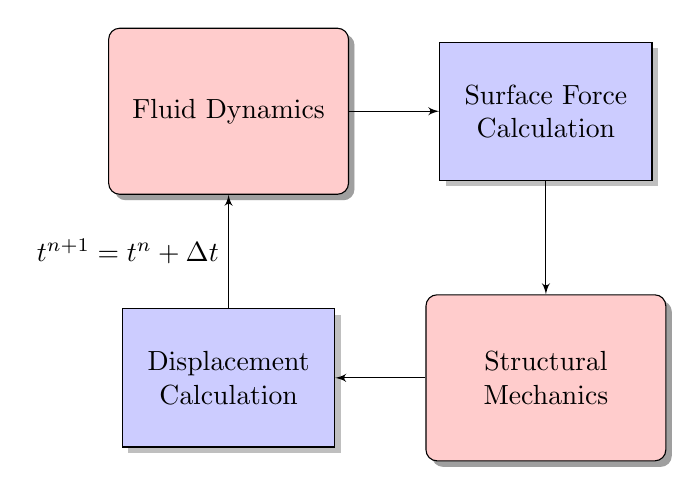
\begin{tikzpicture}[node distance=2.5cm,auto,>=latex']
\tikzstyle{int}=[draw, fill=blue!20, minimum size=2em]
\tikzstyle{init} = [pin edge={to-,thin,black}]

\tikzstyle{sensor}=[draw, fill=blue!20, text width=7em, 
text centered, minimum height=5em,drop shadow]
\tikzstyle{ann} = [above, text width=5em, text centered]
\tikzstyle{wa} = [sensor, text width=8em, fill=red!20, 
minimum height=6em, rounded corners, drop shadow]
\tikzstyle{sc} = [sensor, text width=13em, fill=red!20, 
minimum height=10em, rounded corners, drop shadow]

\node (wa) [wa]  {Fluid Dynamics};
\path (wa.east)+(+2.5,0) node (force) [sensor] {Surface Force Calculation};
\path [draw, ->] (wa.east)  -- node [] {}  (force.west);
\path (force.south)+(0,-2.5) node (structure) [wa] {Structural Mechanics};
\path [draw, ->] (force.south)  -- node [] {}  (structure.north);
\path (structure.west)+(-2.5,0) node (disp) [sensor] {Displacement Calculation};
\path [draw, ->] (structure.west)  -- node [] {}  (disp.east);
\path [draw, ->] (disp.north)  -- node [] {$t^{n+1}=t^{n}+\Delta t$}  (wa.south);
\end{tikzpicture}
\caption{Schematic showing the two-way coupling between the structure and fluid systems.}
\label{fig:FSI}
\end{figure}



\section{Results and Discussion}\label{sec:results}
The Eulerian and Lagrangian approaches are compared and contrasted using four tests. The first test pertains the flow around a cylinder, a widely used single-phase CFD benchmark problem. A dam break test is used to gauge performance for free-surface flows. Lastly, the two approaches are compared in conjunction with two FSI problems -- one pertaining a floating rigid body and one that has the fluid interacting with an elastic/deformable gate. 

\subsection{Flow around cylinder}
\label{subsec:flowAroundCylinder}
This single-phase, internal flow test is used to compare the FE and SPH solutions for a benchmark problem where the flow is shaped by the interplay between the pressure gradient, and the viscous and body forces. The cylinder of radius 0.05\si{m} is positioned at the center of a rectangular domain of height 0.4\si{m} and length 1.0\si{m}. No-slip boundary conditions are applied to the top and bottom walls while periodic (cyclic) conditions are maintained at the left (inlet) and right (outlet) patches. A constant body force $\mathbf{f}_b$=1.0\si{m/s^2} is applied in order to balance the viscous force. The density and viscosity are set to $\rho_0$=10.0\si{kg/m^3} and $\mu$=0.1\si{Pa.s}, respectively. As illustrates in Fig~\ref{fig:FoCV}, the steady-state {\textit{velocity}} predicted by SPH and FEM are qualitatively in close agreement. Note that the difference in the appearance of the plots is not quantitative. Indeed, the ``dotted-like'' look of the SPH plots is a consequence of the Lagrangian nature of the SPH solution in which field values (velocity, in this case) are provided at the location of markers that convect with the flow. Note that the FEM and SPH pressure profiles also show close agreement as illustrated in Fig.~\ref{fig:FoCP}.
\begin{figure}[H]
	\centering	
	\begin{subfigure}{0.45\columnwidth}	
		\centering
		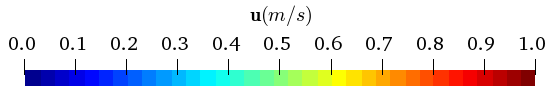
\includegraphics[width=1.0\textwidth]{Images/FOC_U.png}
	\end{subfigure}
	
	\begin{subfigure}{0.47\columnwidth}	
		\centering
		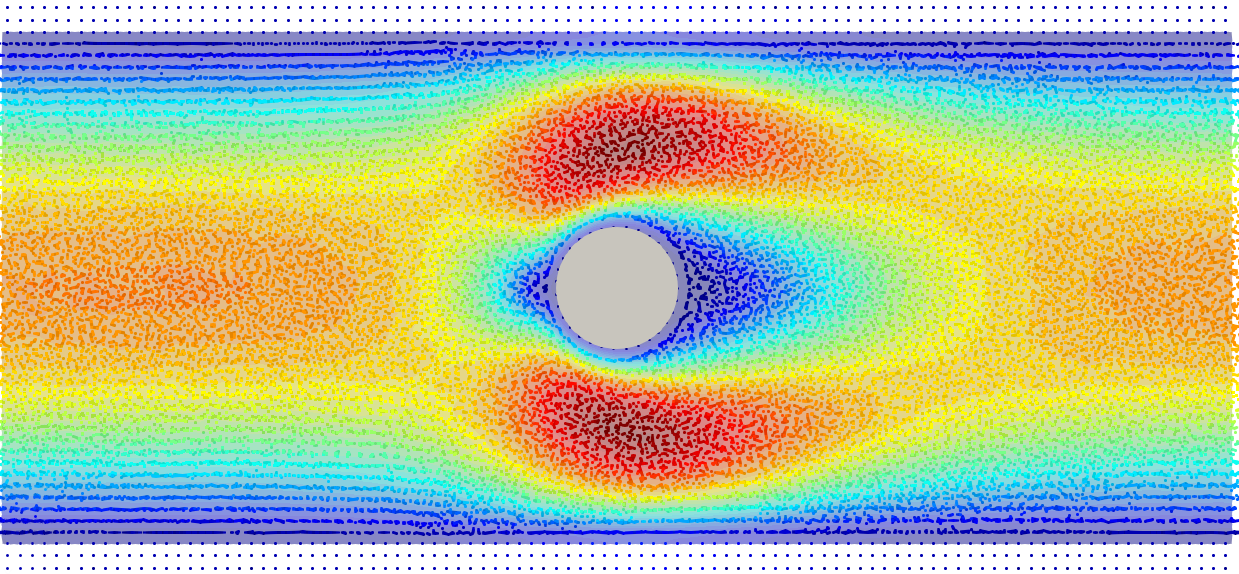
\includegraphics[width=1.0\textwidth]{Images/FOC_SPH_U.png}
	\end{subfigure}
	\begin{subfigure}{0.47\columnwidth}
		\centering
		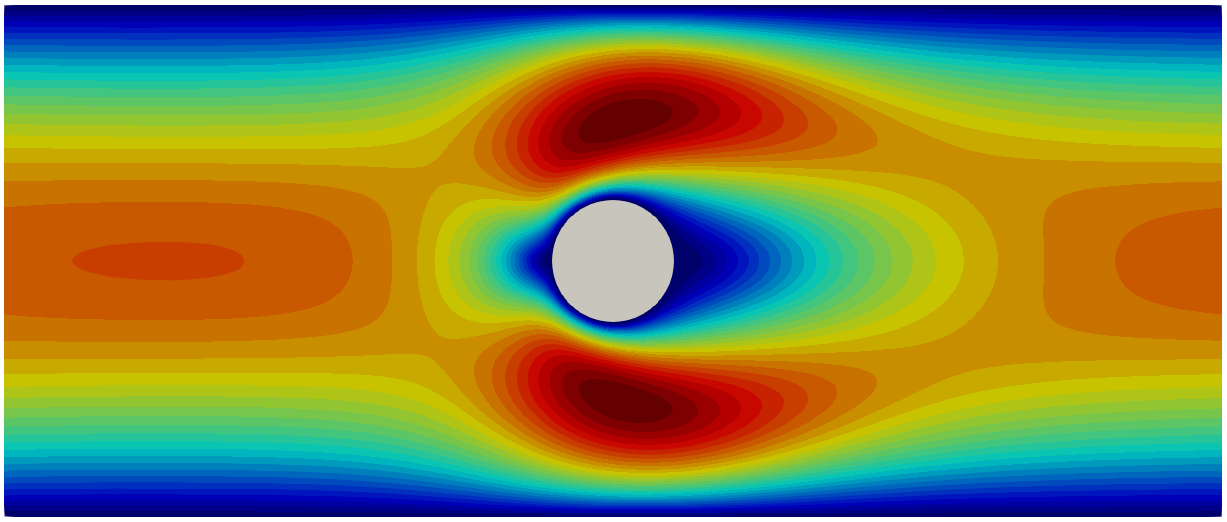
\includegraphics[width=1.0\textwidth]{Images/FOC_FEM_U.png}
	\end{subfigure}
	\caption{Comparison of the steady-state velocity profiles predicted with SPH (left) and FEM (right). The SPH markers outside the fluid domain are BCE markers, see \S\ref{subsec:BC-LagModel}.}	\label{fig:FoCV}
\end{figure} 
% Obtaining the correct smooth pressure field in SPH is generally a more challenging task than in FEM. In Weakly Compressible types of SPH, this is manifested in severe checker-boarding patterns in the pressure field, which happens due to the use of a stiff equation of state for pressure as well as the decoupling of pressure and velocity fields. Historically, the checker-boarding artifact has been fixed in Eulerian methods such as FD method by using \textit{staggered} grids. In staggered grids, the scalar field variables are stored in cell centers while the velocities are stored at the cell faces. This artifact is overcome in FV method by Rhie-Chow type of methods which make it possible to use \textit{collocated} grids as opposed to staggered ones. FE overcomes this artifact by requiring a mixed FE space seen in the Taylor\-Hood elements, in which lower order approximation space is used for pressure comparing to velocity.  Our implicit SPH formulation although is more robust than WCSPH in terms of handling the checker-boarding effects, it still may show this artifact in highly transient problems where the density of individual particles drops below the rest density. In such cases the free-surface boundary condition for pressure ($p=0$) kicks in and causes a zigzaggy pressure field in the neighborhood of the particles with low density.

\begin{figure}[H]
	\centering
		\begin{subfigure}{0.45\columnwidth}	
		\centering
		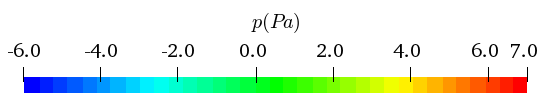
\includegraphics[width=1.0\textwidth]{Images/FOC_p.png}
	\end{subfigure}
	
	\begin{subfigure}{0.47\columnwidth}	
		\centering
		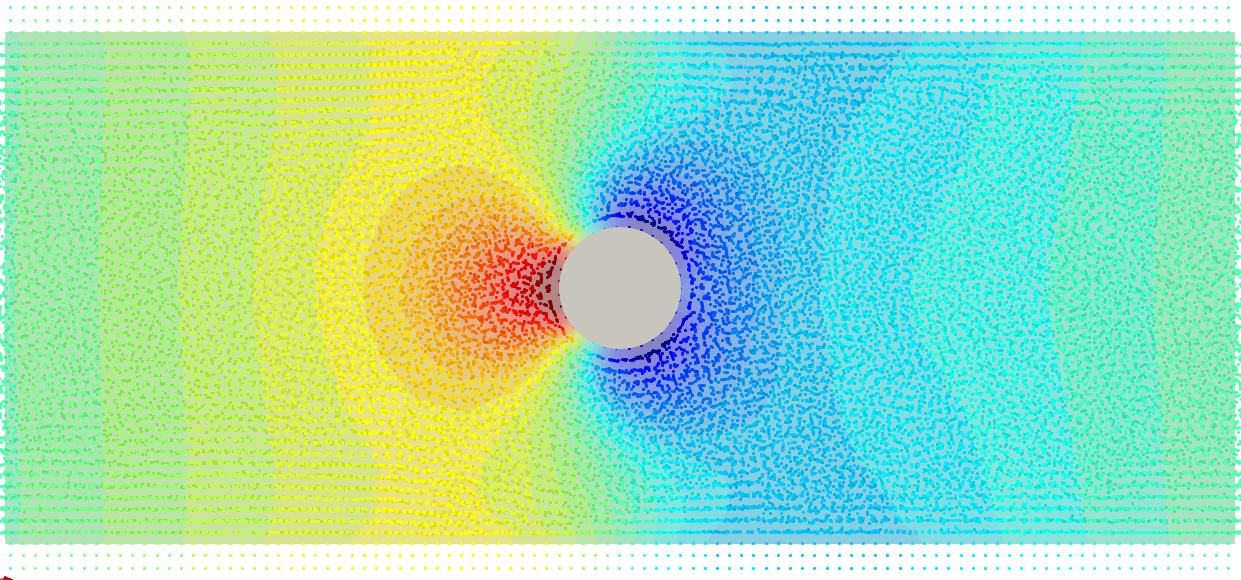
\includegraphics[width=1.0\textwidth]{Images/FOC_SPH_p.png}
	\end{subfigure}
	\begin{subfigure}{0.47\columnwidth}
		\centering
		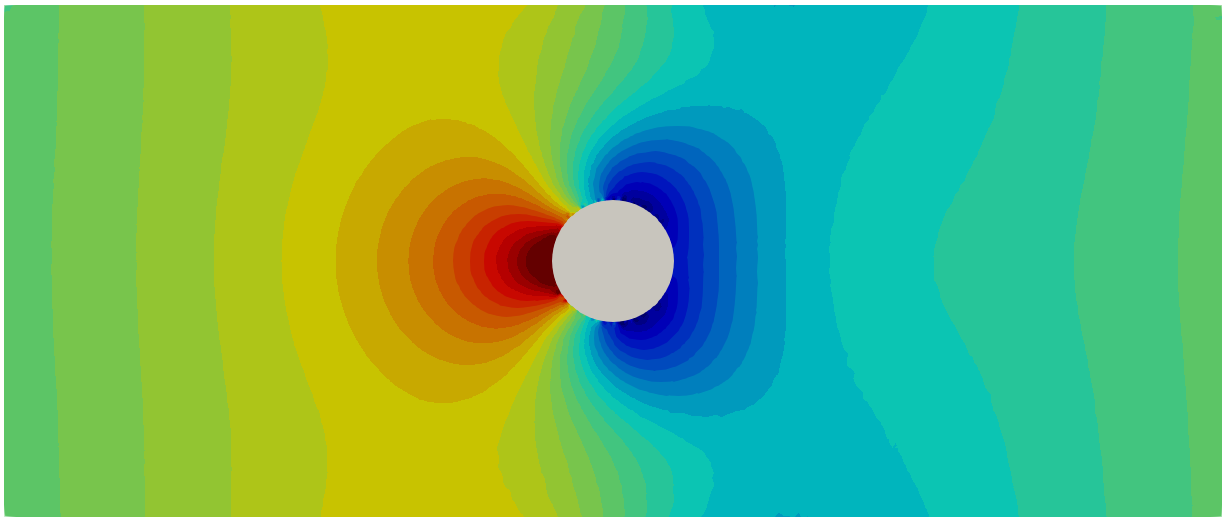
\includegraphics[width=1.0\textwidth]{Images/FOC_FEM_p.png}
	\end{subfigure}
	\caption{Comparison of the steady-state pressure profiles predicted with  SPH (left) and FEM (right). }	\label{fig:FoCP}
\end{figure} 
Lastly, we compare the two methods in terms of drag force. For the drag coefficient, the expression used is $C_d=\frac{F_d}{0.5\rho\;A\; U^2}$, where $F_d$ is the drag force magnitude along the $x$ axis, $\rho=\rho_0$ and $U=1$\si{m/s} are the reference density and velocity, and $A$ is the frontal area of the cylinder.  As shown in Fig.~\ref{fig:FoC}, SPH and FEM show different drag coefficients at the onset of the simulation yet the steady state solutions are in good agreement-- the relative error of the time-averaged drag coefficient over the last 2\si{s} of the simulations is $6.4$\%. We posit that two reasons contributing to these discrepancies are: ($i$) the different time-integration schemes, and ($ii$) the vastly different space discretization technique and boundary condition enforcement used in the formulations. The IB method requires a fine mesh near the solid level-set (cylinder) for accurate representation of the fluid-structure interface and forces. Handling this interface poses no major challenge to SPH or boundary-fitted mesh-based approaches, owing to the explicit representation of the fluid-structure interface.

\begin{figure}[H]
	\begin{center}
        \vspace{-10pt}
		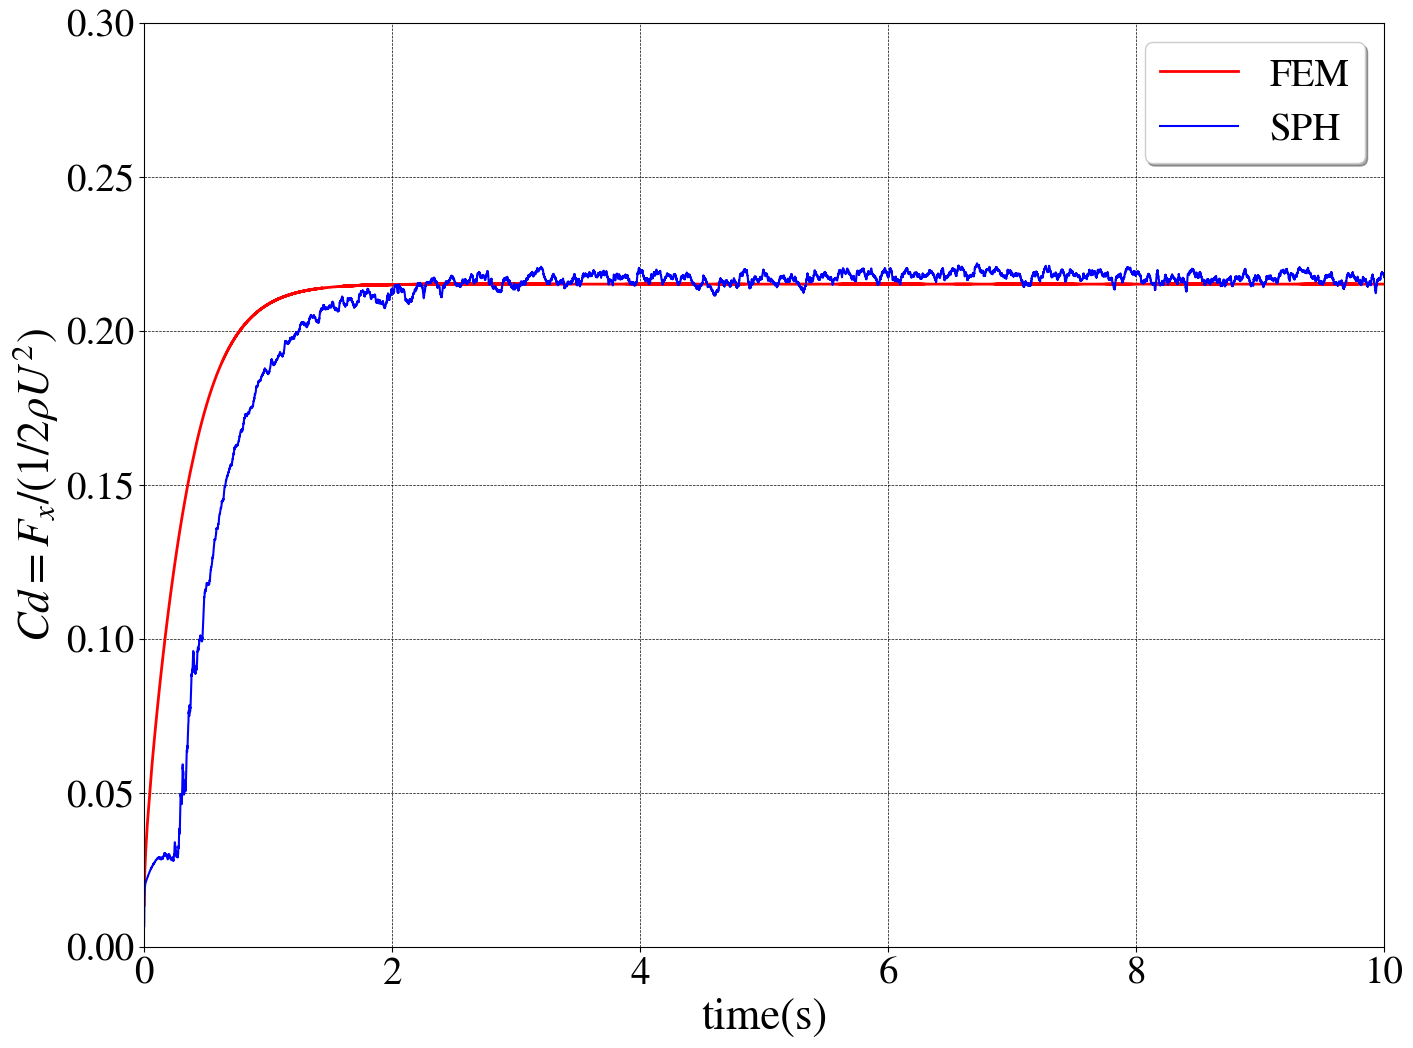
\includegraphics[width=0.5\textwidth]{Images/Figure_flow_around_cylinder.png}
	\end{center}
	\caption{Flow around a cylinder -- variation of the drag coefficient over time.}
	\label{fig:FoC}
%    \vspace{-20pt}
\end{figure}


\subsection{Dam break}
This free-surface flow experiment is setup as follows: the fluid domain is a rectangular prism of size 2\si{m} $\times$ 1.0\si{m}. The reference density and viscosity are $\rho=1000$\si{kg/m^3} and $\mu=$\SI{0.001}{Pa.s}. The gravity $g=-9.8$\si{m/s^2} is applied in the  $y$ direction. The SPH and FEM results are compared from two perspectives: $(i)$ the fluid front position over time, and $(ii)$ the roll up and the second splash -- two characteristics highlighted in previous studies \cite{colagrossi2003numerical,Adami2012}. As shown in Fig.~\ref{fig:db_front}, the SPH solution of the fluid front position over time slightly under-estimate the FEM solution. SPH has an easier task in handling free-surface since in the Lagrangian framework solving the Navier-Stokes equation (Eq.~\eqref{eq:NS}) automatically provides for a tracking of the free-surface  \cite{Martin1952,colagrossi2003numerical,hughes2010comparison,xu2016improved,miladHalfImplicit2018}. In contrast, the Eulerian framework calls for four additional equations: ($i$) the advection of the level-set field via the velocity (Eq.~\eqref{eq:ls_transport_1}); ($ii$) the conservation of the volume fraction (Eq.~\eqref{eq:ls_transport_2}); ($iii$) level-set correction  (Eq.~\eqref{eq:reinitialization}); and ($iv$) the mass correction (Eq.~\eqref{eq:mass_correction}). This adds significantly to the complexity of the Eulerian solution, a drawback that might be eliminated in the future given that very recent work demonstrates that this multistage algorithm can be collapsed into a single stage \cite{quezadadeluna2019monolithic}. 

\begin{figure}[H]
	\begin{center}
		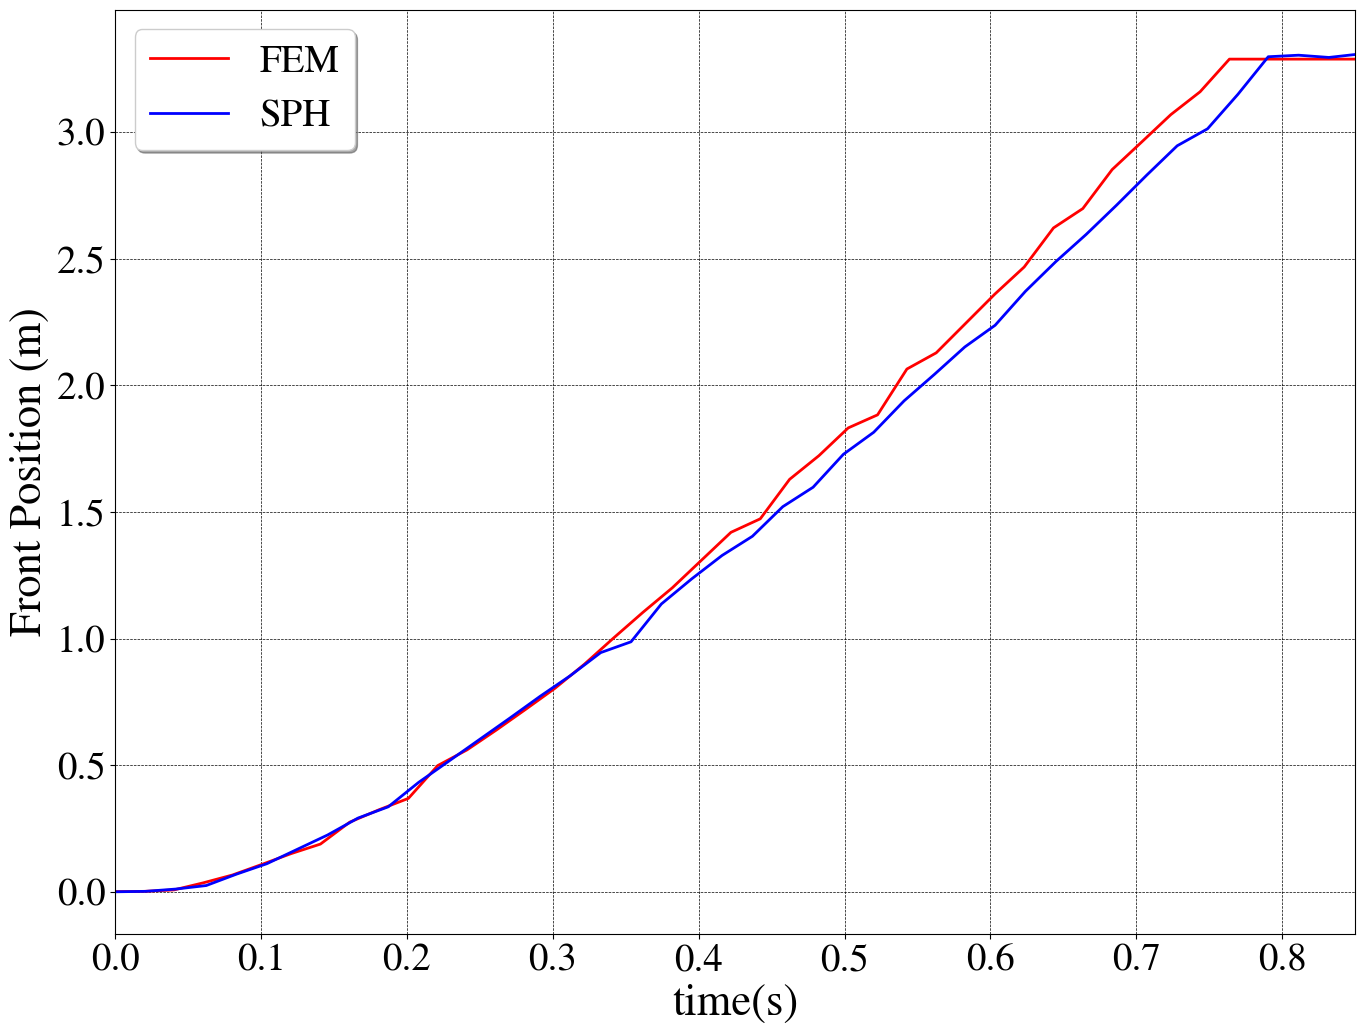
\includegraphics[width=0.5\textwidth]{Images/Figure_damBreak.png}
	\end{center}
	\caption{Comparison of fluid-front propagation between SPH and FEM.}
	\label{fig:db_front}
\end{figure}
With regard to the roll-up and second splash characteristics, both methods predict well these two hallmark features of the dam break experiment, see Fig.~\ref{fig:db_charac}, where the results reported are \SI{1.75}{} and \SI{2.05}{s} into the simulation.
\begin{figure}[H]
	\centering	
		\begin{subfigure}{0.35\columnwidth}	
		\centering
		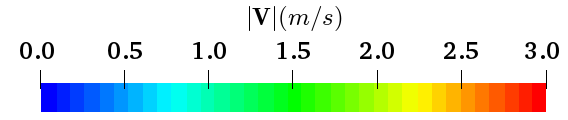
\includegraphics[width=1.0\textwidth]{Images/DB_U.png}
	\end{subfigure}

	\begin{subfigure}{0.4\columnwidth}	
		\centering
		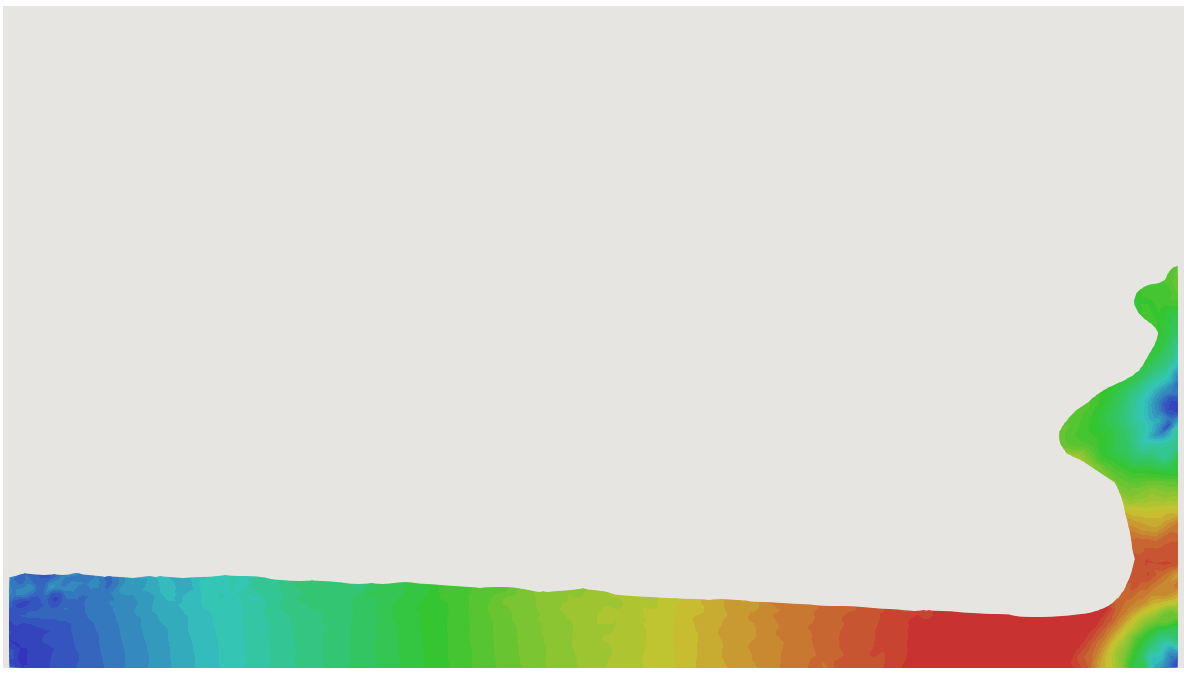
\includegraphics[width=1.0\textwidth]{Images/DB_FEM_1.png}
	\end{subfigure}
	\begin{subfigure}{0.4\columnwidth}
		\centering
		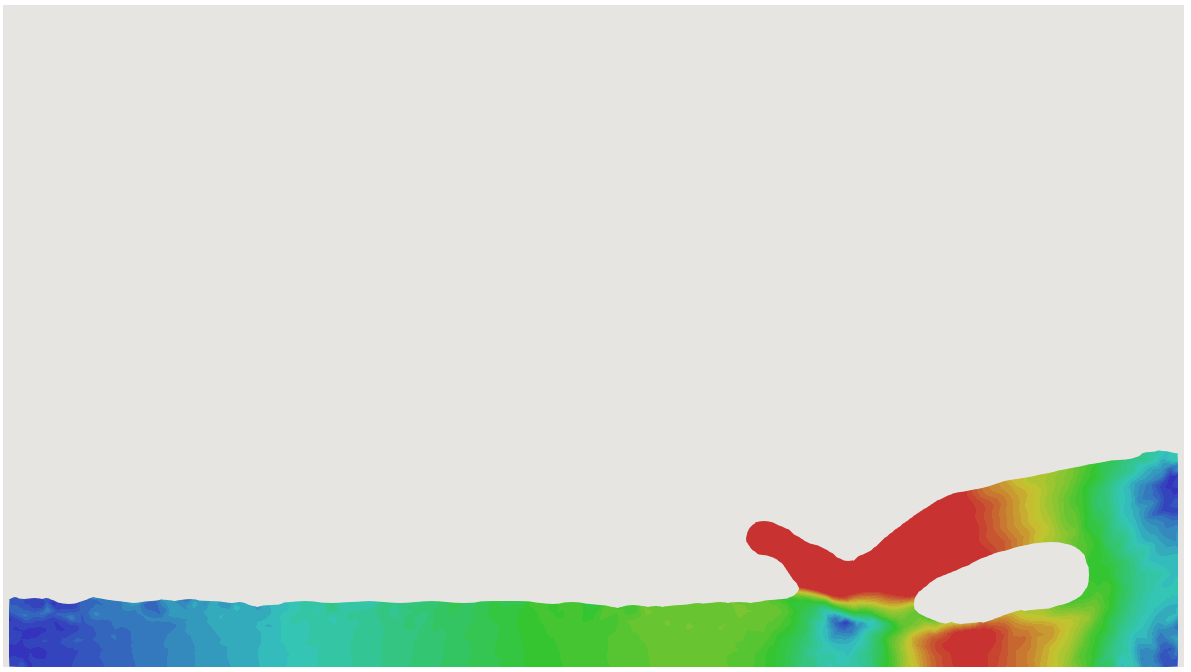
\includegraphics[width=1.0\textwidth]{Images/DB_FEM_2.png}
	\end{subfigure}
	\begin{subfigure}{0.4\columnwidth}	
	\centering
	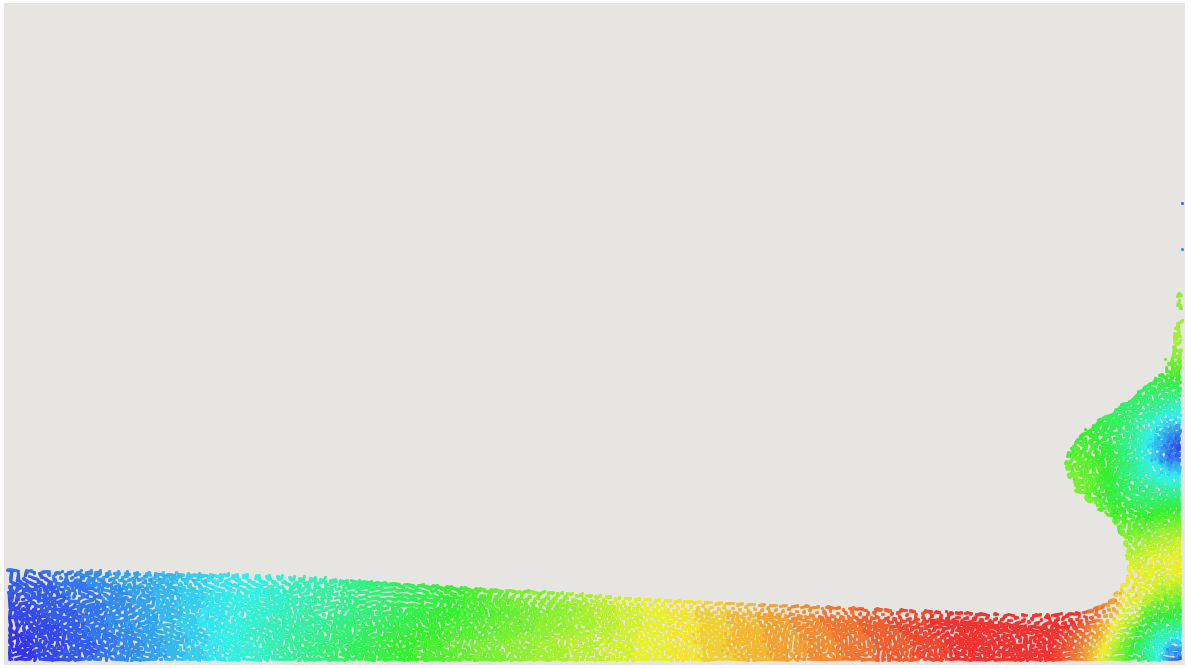
\includegraphics[width=1.0\textwidth]{Images/DB_SPH_1.png}
	\end{subfigure}
	\begin{subfigure}{0.4\columnwidth}
		\centering
		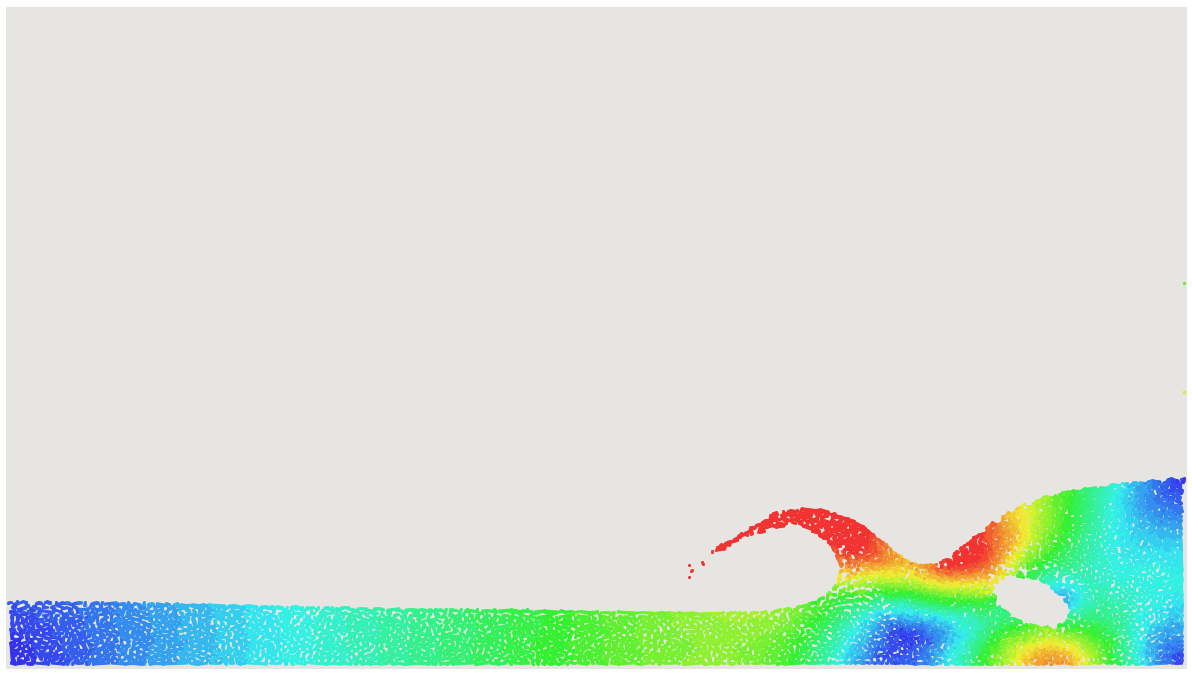
\includegraphics[width=1.0\textwidth]{Images/DB_SPH_2.png}
	\end{subfigure}
	\caption{Comparison of the roll-up ($t=1.75$\si{s}, left) and the second splash ($t=2.05$\si{s}, right) for the dam break -- FEM (top) and SPH (bottom).}	
    \label{fig:db_charac}
\end{figure}

\subsection{Fluid Interaction with a Falling Cylinder}
This experiment was used to compare the Eulerian and Lagrangian approaches in conjunction with a 3D scenario that displayed ample fluid-solid boundary movement. It may be regarded as a simplified problem that, in more complex forms, is conspicuous in several fluid-structure interaction applications in coastal and offshore structures, e.g., renewable energy devices and caissons. Insofar as the solution methodology is concerned, the test assesses the robustness of the fluid-structure coupling methodology described in \ref{sec:FSI}. 

The problem is setup as follows. A cylindrical object of radius $r=0.12$\si{m} and length $L=0.2$\si{m} is released from the height $h=0.25$\si{m} above the surface of a tank of water at $t=0$\si{s}. The dimension of the fluid domain is 1.0\si{m} $\times$ 1.0\si{m} $\times$ 0.2\si{m} (width$\times$height$\times$depth). The gravity $g=-9.8$\si{m/s^2} is applied in the $y$ direction. The reference density and viscosity of the water are $\rho=1000$\si{kg/m^3} and $\mu=$\SI{0.001}{Pa.s}. The density of the cylinder is $\rho_s=0.7\rho$, which turns it into a floating structure. Figure~\ref{fig:CD} illustrates the distribution of the pressure in the frontal cross-section of the domain at $t=0.5$\si{s}. 

The cylinder oscillates until its initial potential energy damps out. The {\textit{steady-state}} solution of this problem is given by Newton's second law and basic hydrostatics. Indeed, the upward buoyant force exerted on the body should balance the weight of the object; i.e., $\rho_s g V =62.0$. Figure~\ref{fig:CD_F} illustrates the vertical component of the fluid-structure interaction forces obtained with FEM and SPH and the fact that both methods close in on the stead-state solution approximately \SI{6}{s} into the simulation. Although the two models show similar characteristics and steady-state configuration for the vertical force, the SPH solution damps out the oscillation faster due to $(i)$ more numerical damping, and more importantly, $(ii)$ tighter connection between the fluid and the structure degrees of freedom demonstrated by denser system matrices. Specifically, the FEM fluid-structure force uses the \textit{smoothed} Heaviside and Dirac delta functions (see Eq.~\eqref{eq:approx_H}). This smoothing is numerically done along $h_e<\epsilon<2h_e$ in the mesh where $h_e$ is the elements' characteristic length scale. Incorporating the information from nodes further away at any point require increasing this smoothing length, which consequently deteriorates the accuracy of the numerical fluid-structure forces.
\begin{figure}[H]
	\centering
	\begin{subfigure}{0.38\columnwidth}	
		\centering
		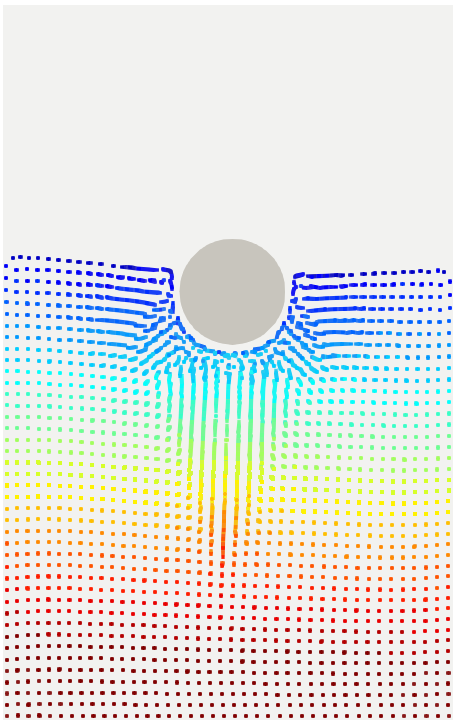
\includegraphics[width=1.0\textwidth]{Images/CD_SPH.png}
	\end{subfigure}
	\begin{subfigure}{0.38\columnwidth}
		\centering
		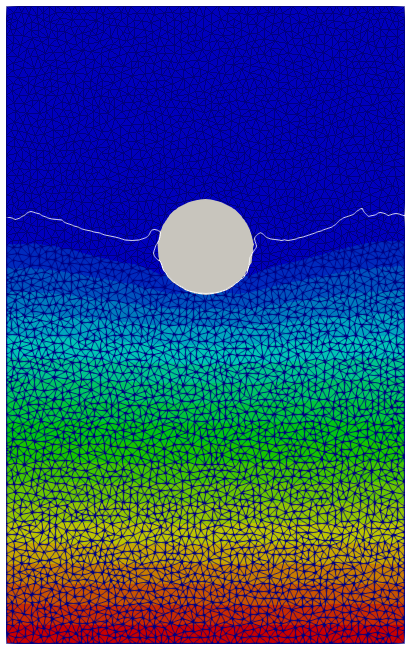
\includegraphics[width=1.0\textwidth]{Images/CD_FEM.png}
	\end{subfigure}
	\begin{subfigure}{0.15\columnwidth}	
		\centering
		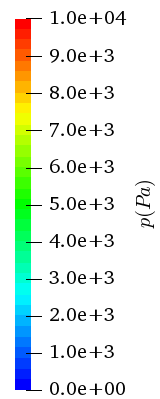
\includegraphics[width=1.0\textwidth]{Images/CD_p.png}
	\end{subfigure}
	\caption{Comparison of the steady-state pressure profiles predicted with  SPH (left) and FEM (right).}	\label{fig:CD}
\end{figure} 

\begin{figure}[H]
	\begin{center}
		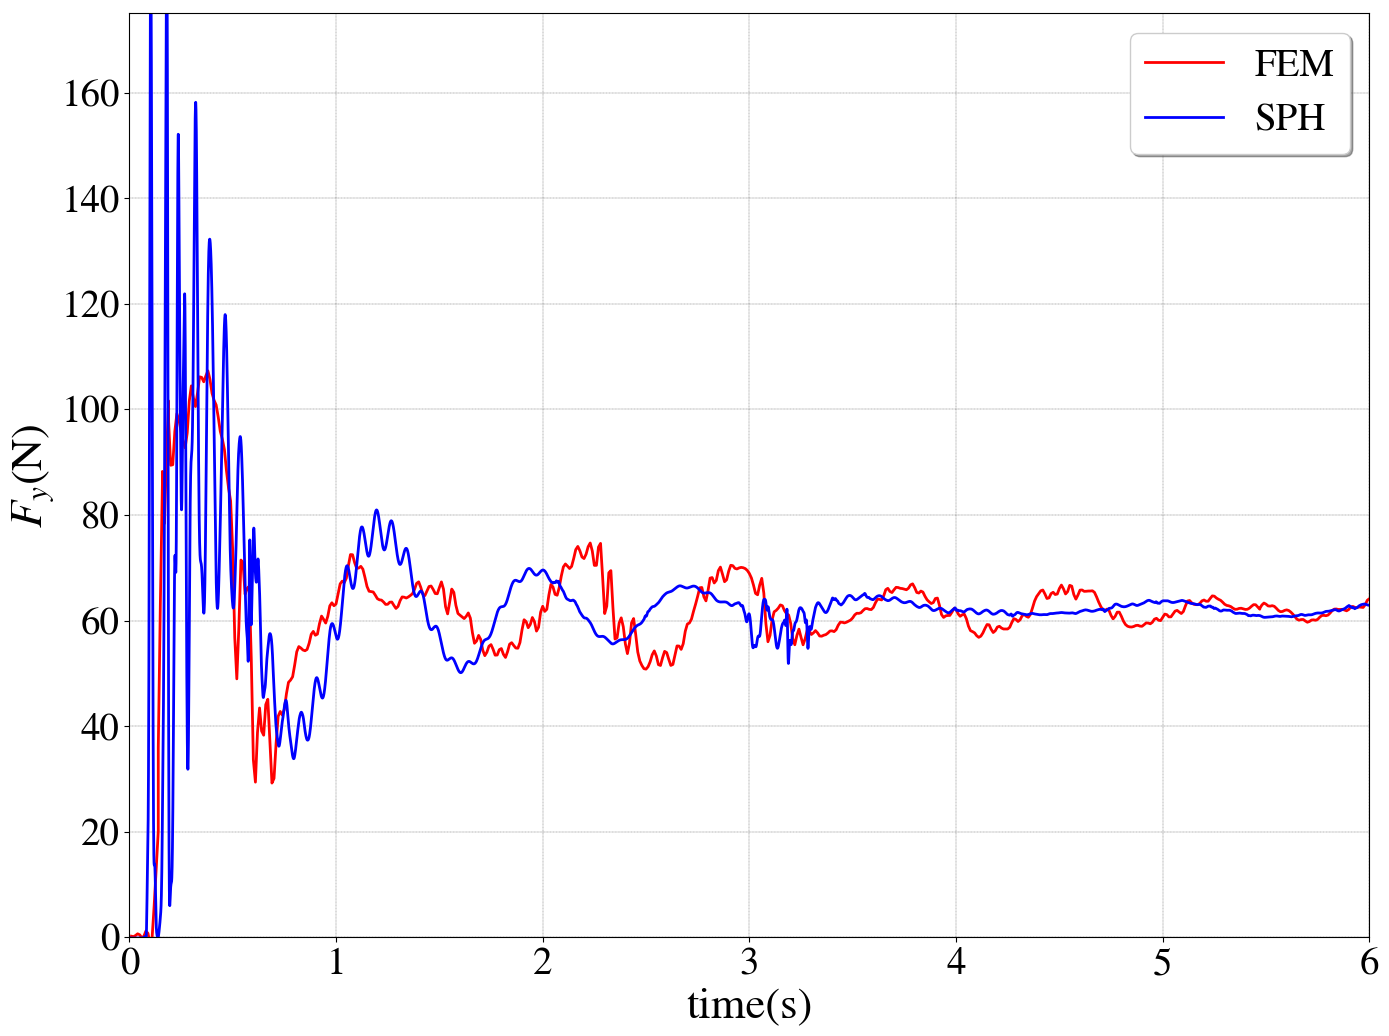
\includegraphics[width=0.5\textwidth]{Images/Figure_Cylinder_FSI.png}
	\end{center}
	\caption{Upward buoyant force imparted  over time by the fluid to the floating cylinder.}
	\label{fig:CD_F}
\end{figure}

\subsection{Flexible Gate}
In this experiment \cite{Antoci2007,yang2012}, water is stored in a cubic container that has three rigid vertical sides while the fourth one is partially made up of a rectangular elastic rubber gate, see the $t=0$ \si{s} schematic in Fig.~\ref{fig:Elastic_Gate_Schematic}. The elastic gate, which experiences large deformations, is simulated using a non-linear finite element method called the Absolute Nodal Coordinate Framework (ANCF) \cite{shabana2013}. The details about the gradient-deficient ANCF element used herein fall outside of the scope of this contribution but may be found in \cite{yamashita2015continuum}. 
\begin{figure}[H]
	\begin{center}
		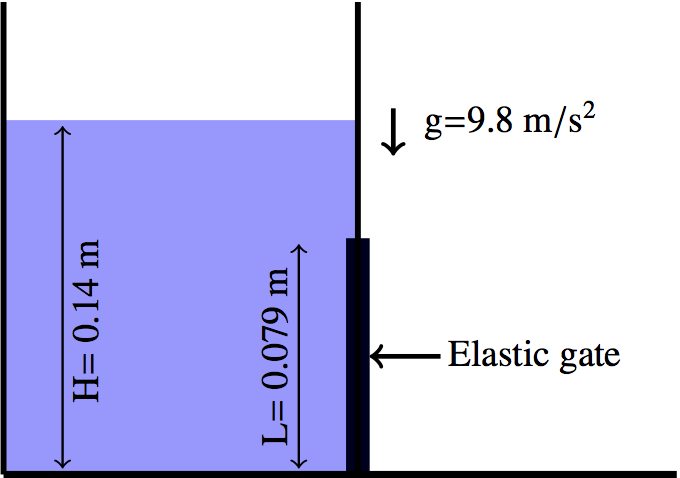
\includegraphics[width=0.32\textwidth]{Images/Elastic_Gate_Schematic.png}
	\end{center}
	\caption{Schematic and specifications of the elastic gate experiment. Fluid properties: $\rho=1000$ \si{kg/m^3}, $\mu=0.001$ \si{Pa}$\cdot$\si{s}. Gate properties: $\rho_s=1100$ \si{kg/m^3}, $E=10$ \si{MPa}, $\nu=0.4$, thickness=0.005 \si{m} \cite{Antoci2007}. }
	\label{fig:Elastic_Gate_Schematic}
\end{figure}


Due to the hydrostatic pressure, the elastic gate gradually deflects and the water exit the tank as shown in Fig.~\ref{fig:EG}.
\begin{figure}[H]
	\centering	
	\begin{subfigure}{0.4\columnwidth}	
		\centering
		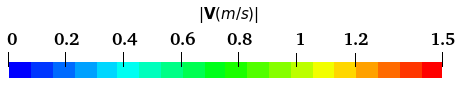
\includegraphics[width=1.0\textwidth]{Images/FSI_colorbar.png}
	\end{subfigure}
	\begin{subfigure}{0.8\columnwidth}	
		\centering
		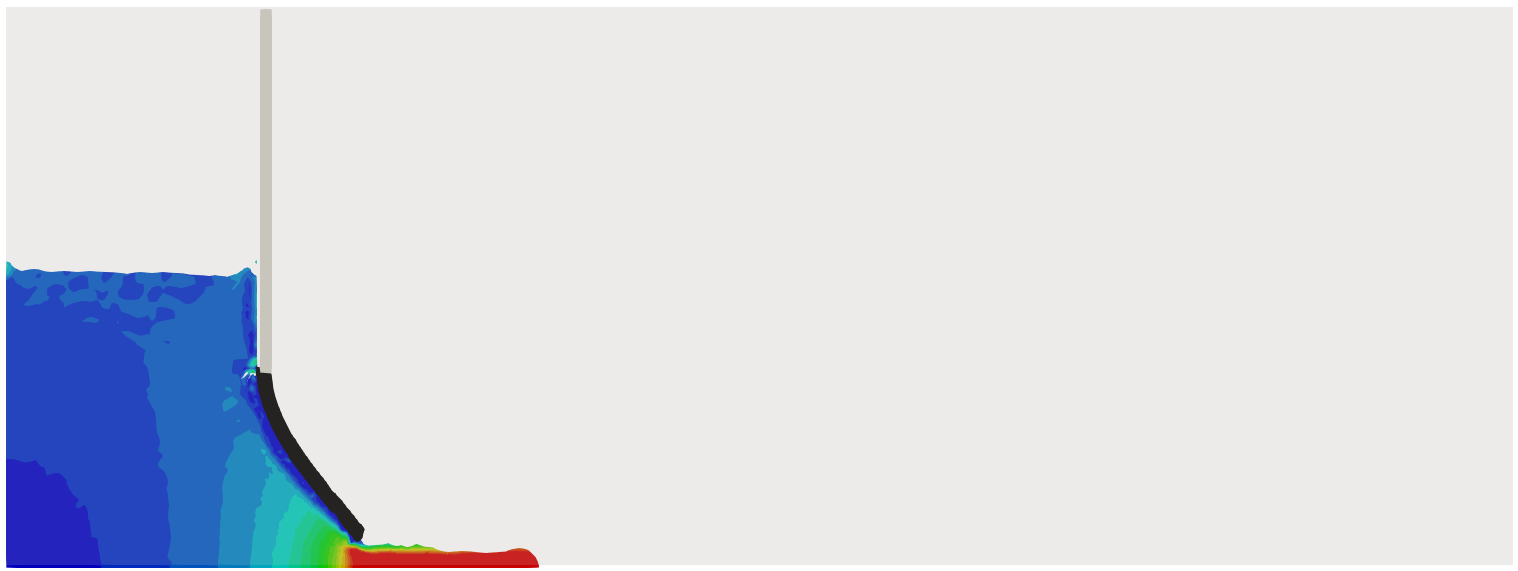
\includegraphics[width=1.0\textwidth]{Images/FSI_FEM.png}
	\end{subfigure}
	\begin{subfigure}{0.8\columnwidth}
		\centering
		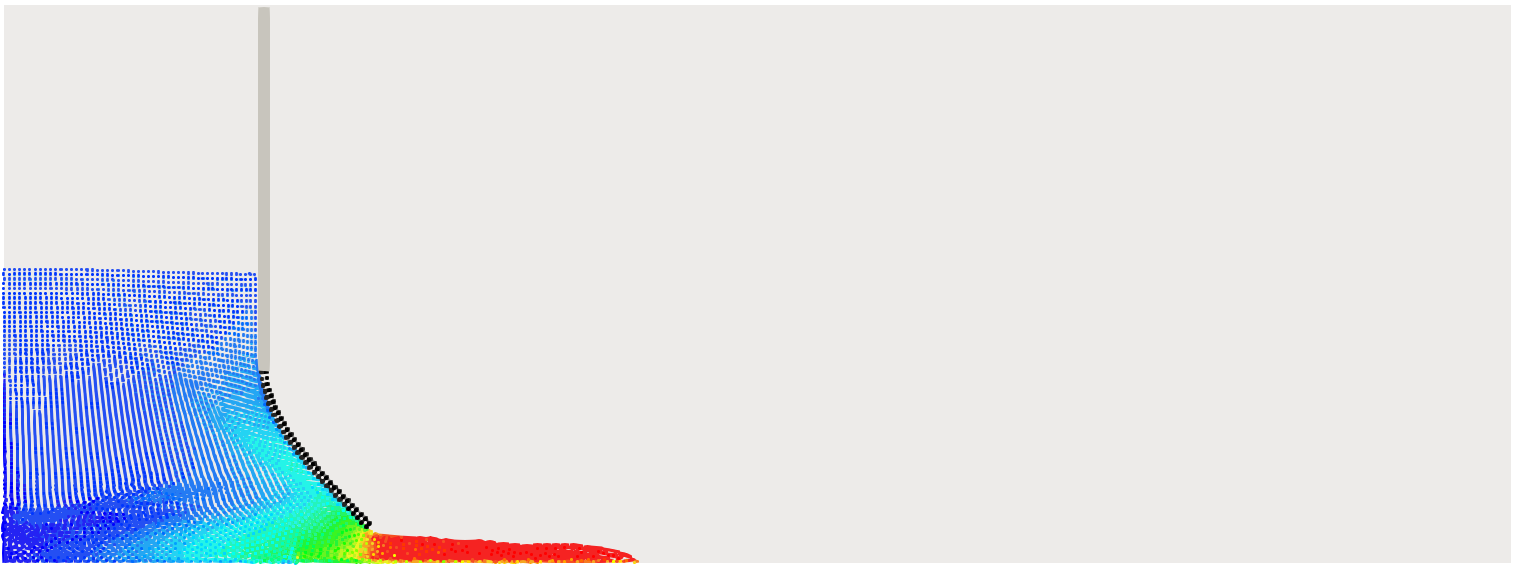
\includegraphics[width=1.0\textwidth]{Images/FSI_SPH.png}
	\end{subfigure}
		\caption{Snapshots of the elastic gate simulation with FEM (top) and SPH(bottom). The fluid domain colored according to velocity magnitude. The $x$ axis is horizontal, pointing to the left; the $y$ axis is vertical, pointing up.}
		\label{fig:EG}
\end{figure} 
The position of the tip of the gate was measured in the experiment reported in \cite{Antoci2007}. The simulation results of both SPH and FEM under-predict the deformation results reported in \cite{Antoci2007} but are consistent with numerical results reported in \cite{yang2012}.
\begin{figure}[H]
    \vspace{-15pt}
	\begin{center}
		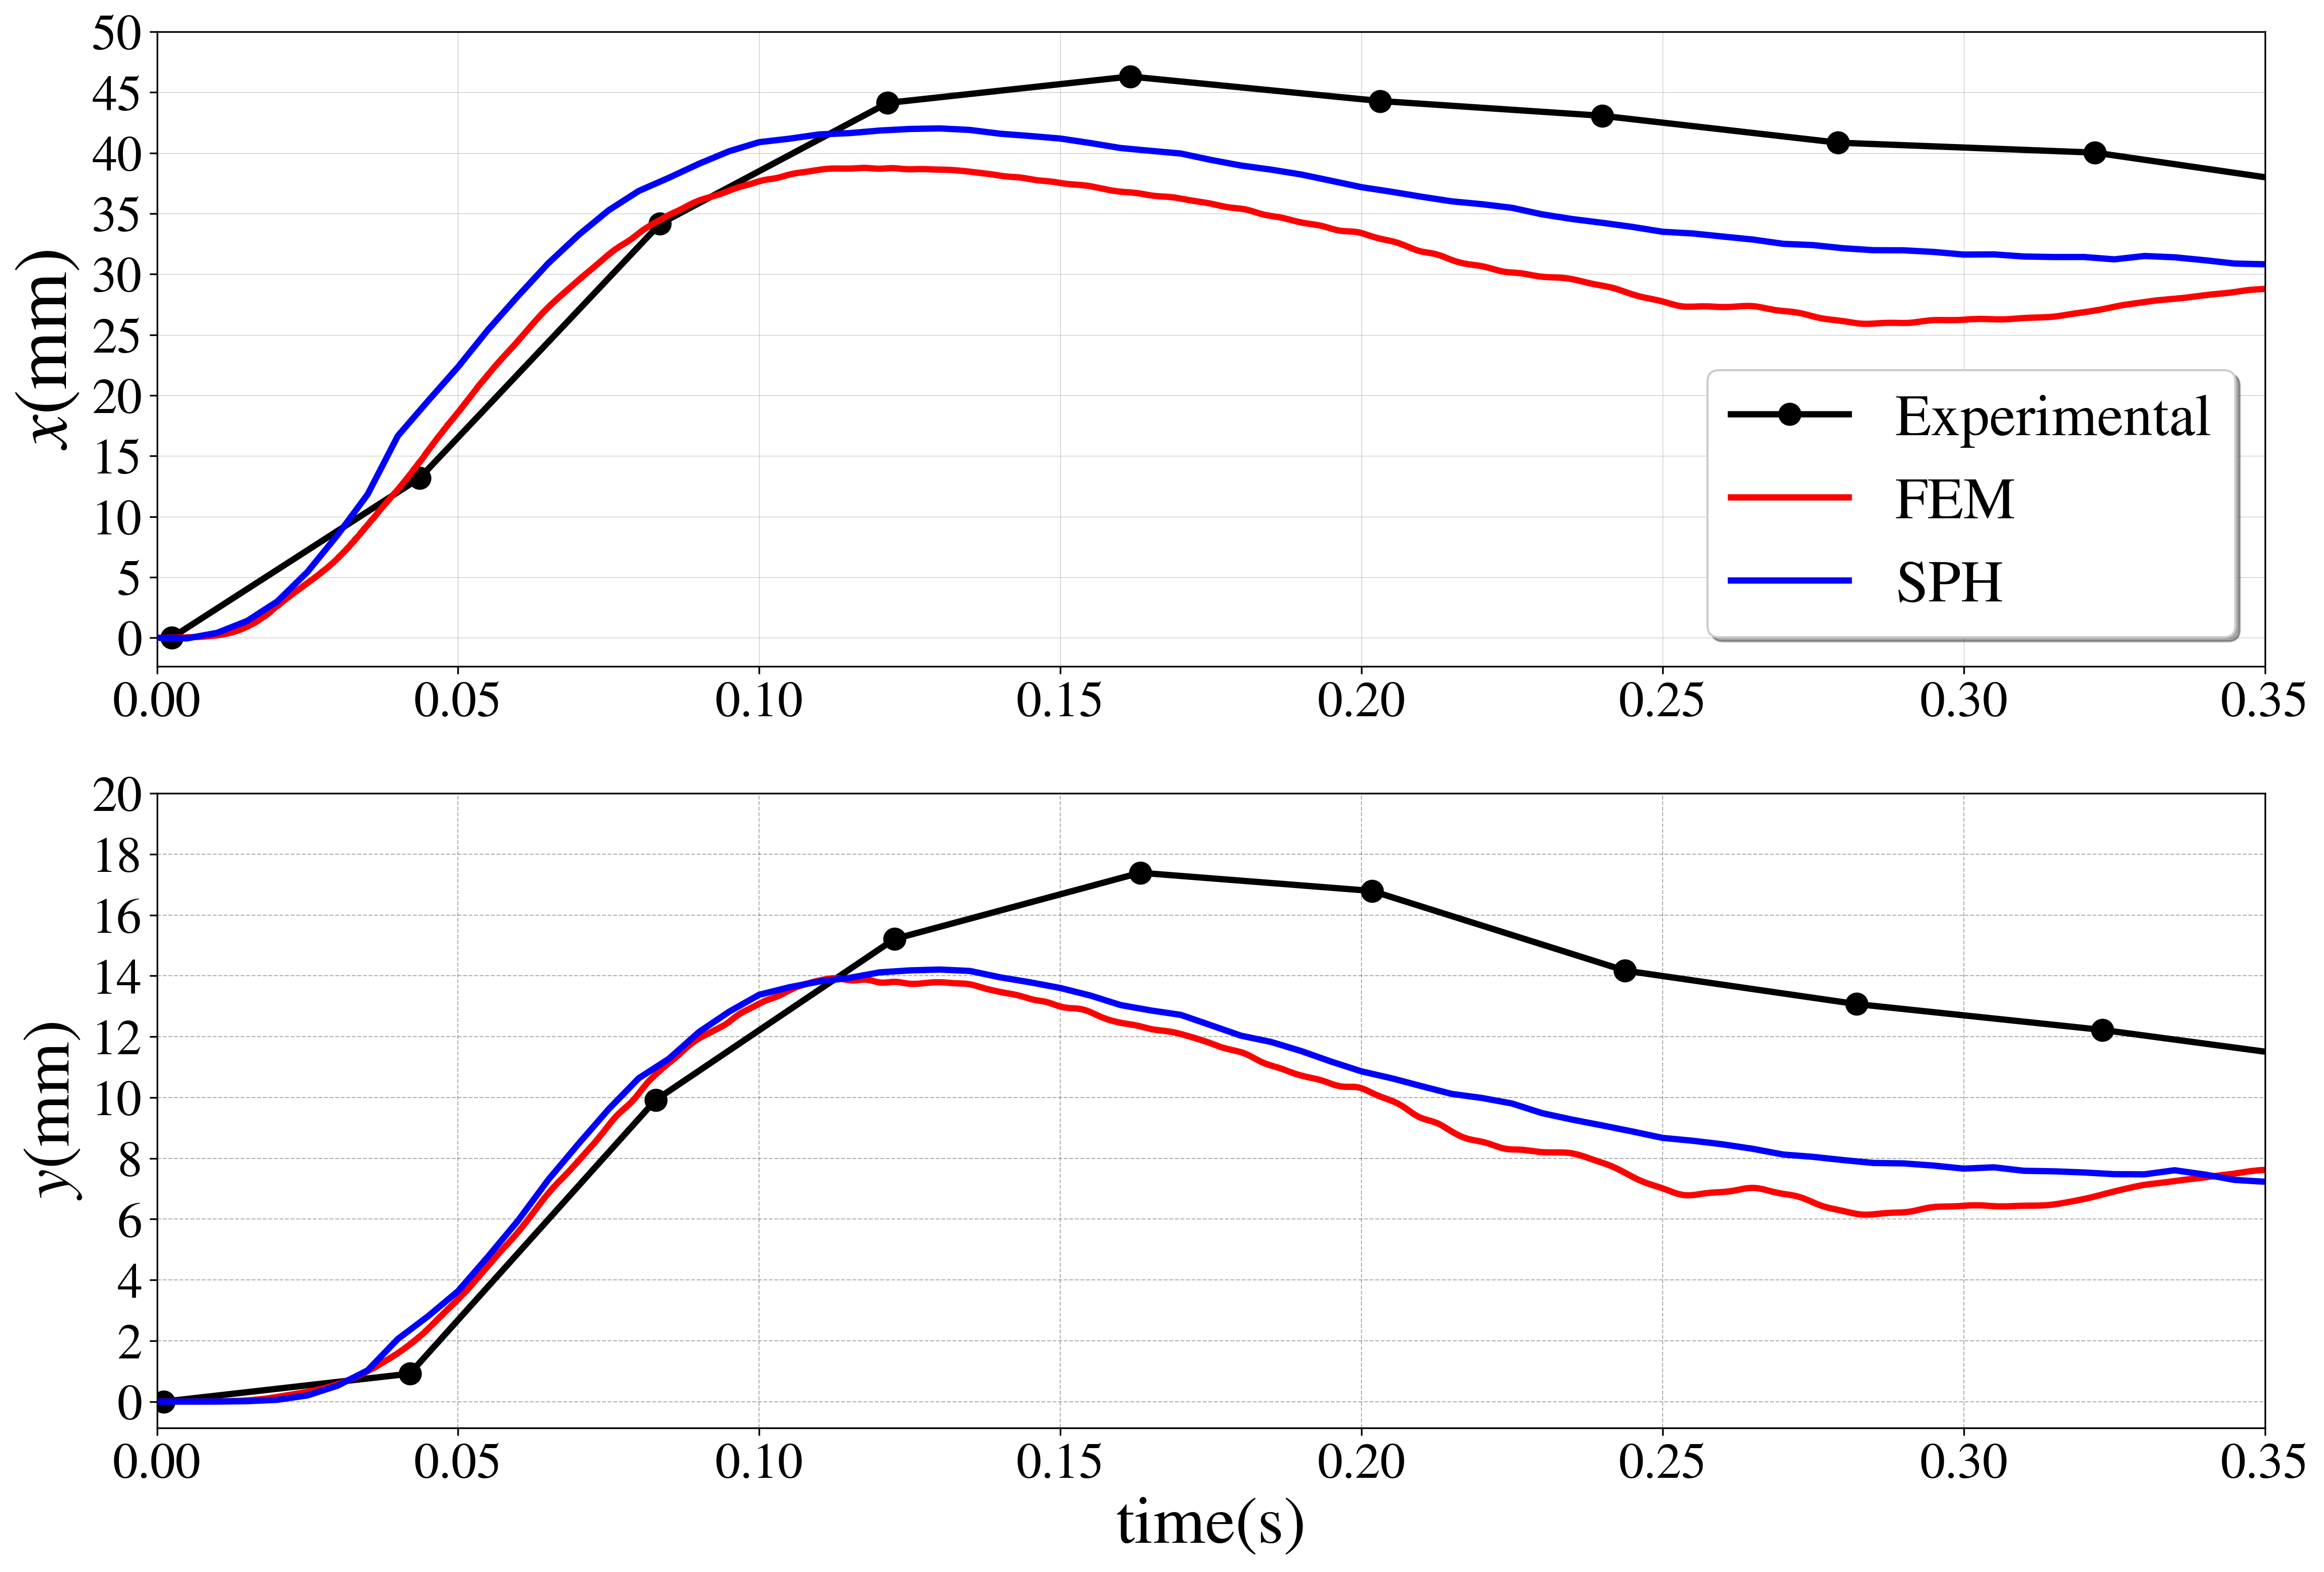
\includegraphics[width=0.5\textwidth]{Images/Fig_FSI.png}
	\end{center}
	\caption{Comparison of the position of the tip of the gate between SPH, FEM and experimental results \cite{Antoci2007}.}
	\label{fig:db_front_flexGate}
\end{figure}


\section{Conclusions}\label{sec:conclusion}
We report results of a study that compared and contrasted the Eulerian and Lagrangian approaches for the solution of free-surface and Fluid-Solid Interaction (FSI) problems. The two approaches are implemented in two open source and publicly available codes -- Proteus and Chrono, which embrace, respectively, FEM-based and SPH-based solutions. Four tests were considered in this study: flow around a cylinder, dam break, falling yet floating cylinder in fluid tank, and elastic gate problems. We conclude that the SPH methodology is permissive and expeditious. When compared to a more robust Eulerian method such as FEM, the GPU parallelized SPH solver delivers a solution that is reasonably accurate, computationally less demanding, and easier to produce for the class of problems investigated in this work.  The FEM solver is more accurate as are the methods it draws on.

Solving fluid-solid interaction problems of practical relevance remains a challenging undertaking that usually draws on the interplay of complex modeling, numerical algorithms, and software solution techniques. In this context, our goal was that of gaining insights into how the Eulerian and Lagrangian approaches dictate the quality of the FSI numerical solution, which touches on ease of simulation setup as well as solver robustness and efficiency. The two solutions considered herein are polar opposites since the dynamics of the fluid phase was resolved via vastly different space and time discretization techniques as well as software implementations. Indeed, the Lagrangian, SPH-based solver in Chrono condenses the non-linear velocity advection term present in the momentum conservation of the Eulerian formulation (Eq.~\eqref{eq:Eulerian_NS}) into the material derivative (Eq.~\eqref{eq:NS}). Moreover, the Lagrangian description (Eqs.~\eqref{eq:predict}-\eqref{eq:correct}) embraced in Chrono renders the system of equations linear with respect to the velocity unknown. Consequently, the most demanding stage of the Chrono implementation calls at each time step for the solution of a linear system for pressure and velocities. In contrast, the FEM solution in Proteus builds off a more involved implementation that considers additional equations that capture the fluid-solid interface; i.e., the level set advection (Eq.~\eqref{eq:ls_transport_1}) and the volume fraction conservation (Eq.~\eqref{eq:ls_transport_2}). Since the solution of Eq.~\eqref{eq:ls_transport_1} does not guarantee that the new level set is a sign distance function, the level set field needs to be re-initialized (Eq.~\eqref{eq:reinitialization}). A mass conservation correction is also required (Eq.~\eqref{eq:mass_correction}). The non-linearity associated with the advection term is resolved by using the previous time-step velocity. Nonetheless, even if a projection method is used to decouple pressure and velocity and linearize the Navier-Stokes equation, the mass conservation equation remains non-linear. All things considered, the FEM solver is more sophisticated and computationally demanding. This is because: $(i)$ more equations need to be solved in the FEM solver, and $(ii)$ the FEM solver calls for the solution of a non-linear system, which requires the derivation of Jacobian and residual terms. Regarding the parallelization of the solvers, the SPH solver leveraged GPU computing through CUDA which is suitable for fine grain parallelization required in SPH. The FEM solver used a distributed memory multi-core parallel implementation via Message Passing Interface (MPI).

The quality of the pressure field was superior in the FEM solution. Obtaining the correct smooth and accurate field in SPH is more challenging. For instance, if one uses the classical weakly compressible SPH solver that is widely employed in the community but was not considered herein, the pressure field will experience severe checker-boarding patterns. This can be traced back to the use of a stiff equation of state for evaluating the pressure field, as well as to the decoupling of the velocity and pressure fields -- aspects that do not plague the implicit SPH solution discussed herein. 
The implicit SPH formulation, although more robust than the weakly compressible alternative, may still show checker-boarding effects in highly transient problems where the density of individual particles drops below the rest density. In such cases the free-surface boundary condition for pressure ($p=0$) kicks in and causes a zigzagging pressure field in the neighborhood of the particles with low density. The checker-boarding artifact has been fixed in Eulerian methods such as the FD method by using staggered grids. The same artifact is avoided on collocated grids in the FV method by Rhie-Chow type algorithms. FE overcomes this artifact by requiring a mixed FE space seen in the Taylor-Hood elements, in which a lower order approximation space is used for pressure compared to velocity.  

Regarding the solution robustness and flexibility, the FEM solver is more robust insofar as the fluid handling is concerned since it takes advantage of the good accuracy and stability of established Eulerian methods. It also allows for a richer set of boundary condition types and flow regimes. On the other hand, the SPH solver in our experience is more robust when dealing with the class of FSI problems studied herein. This is mainly due its Lagrangian framework that lends itself well to the coupling between the fluid and solid phases. 

\section*{Acknowledgment}
This work was partially funded by National Science Foundation grant CMMI-1635004.


\bibliographystyle{plain}
\bibliography{ref}
\end{document}

%%
%% End of file `elsarticle-template-num.tex'.
